% TeX eps-loader file generated by stoch_simul.m (Dynare).
% 05-Mar-2024 16:44:40
 
\begin{figure}[H]
\centering 
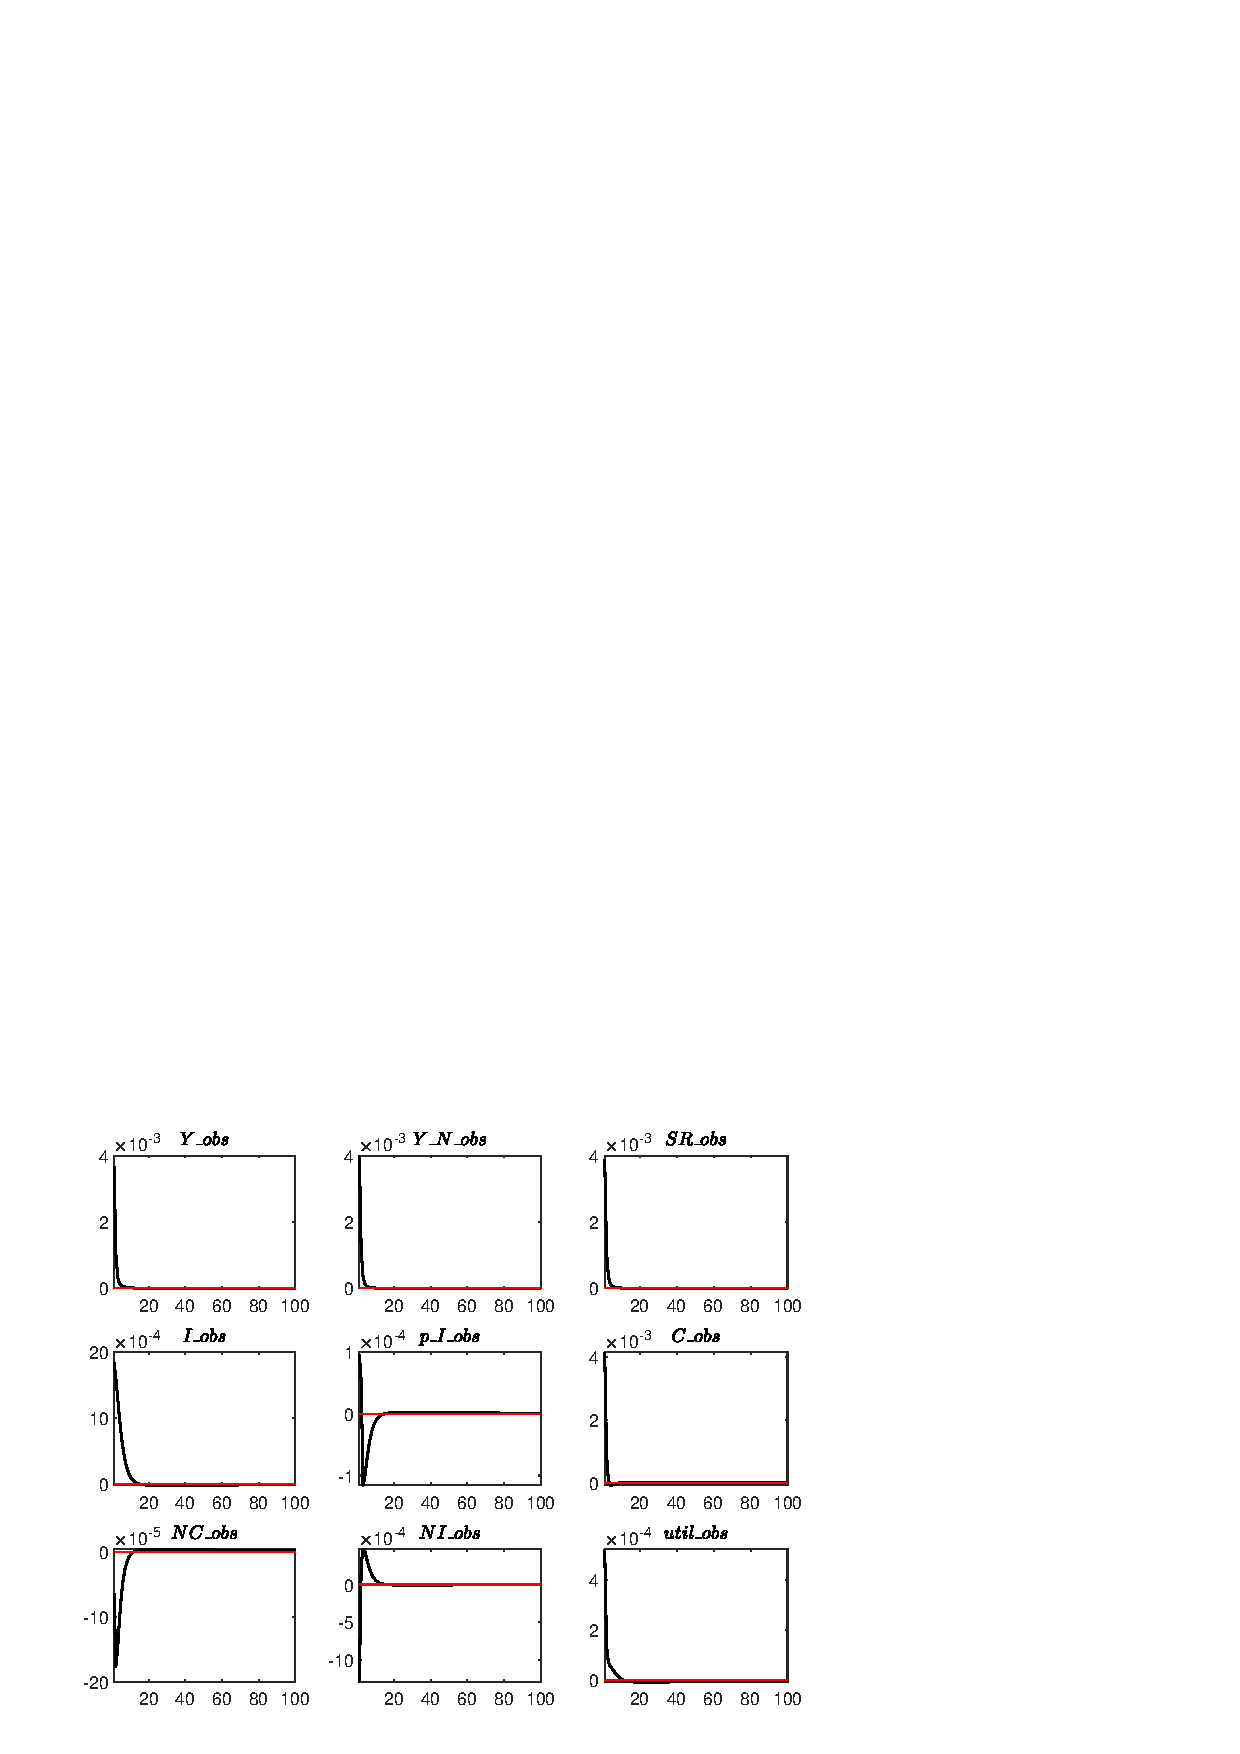
\includegraphics[width=0.80\textwidth]{BRS_growth/graphs/BRS_growth_IRF_e_g1}
\caption{Impulse response functions (orthogonalized shock to ${e_g}$).}\label{Fig:IRF:e_g:1}
\end{figure}
 
\begin{figure}[H]
\centering 
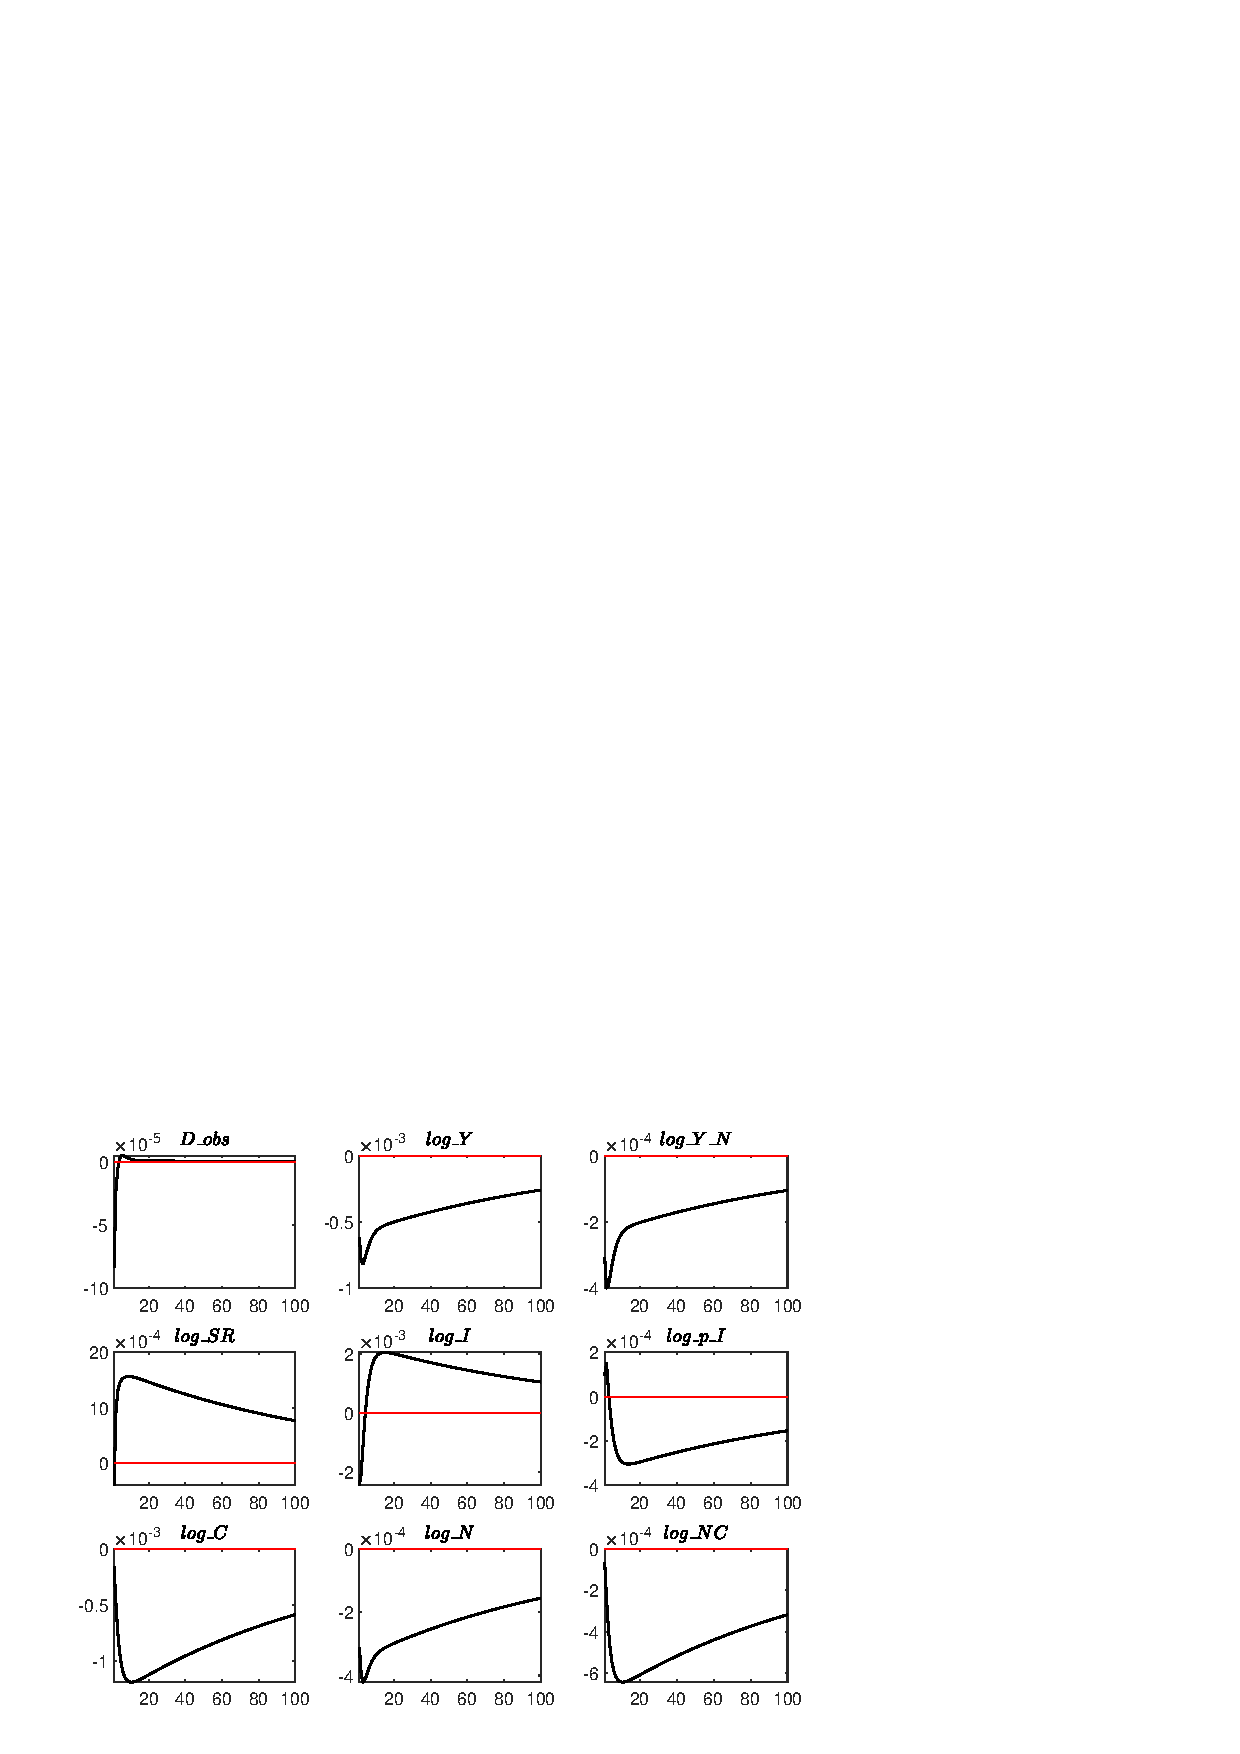
\includegraphics[width=0.80\textwidth]{BRS_growth/graphs/BRS_growth_IRF_e_g2}
\caption{Impulse response functions (orthogonalized shock to ${e_g}$).}\label{Fig:IRF:e_g:2}
\end{figure}
 
\begin{figure}[H]
\centering 
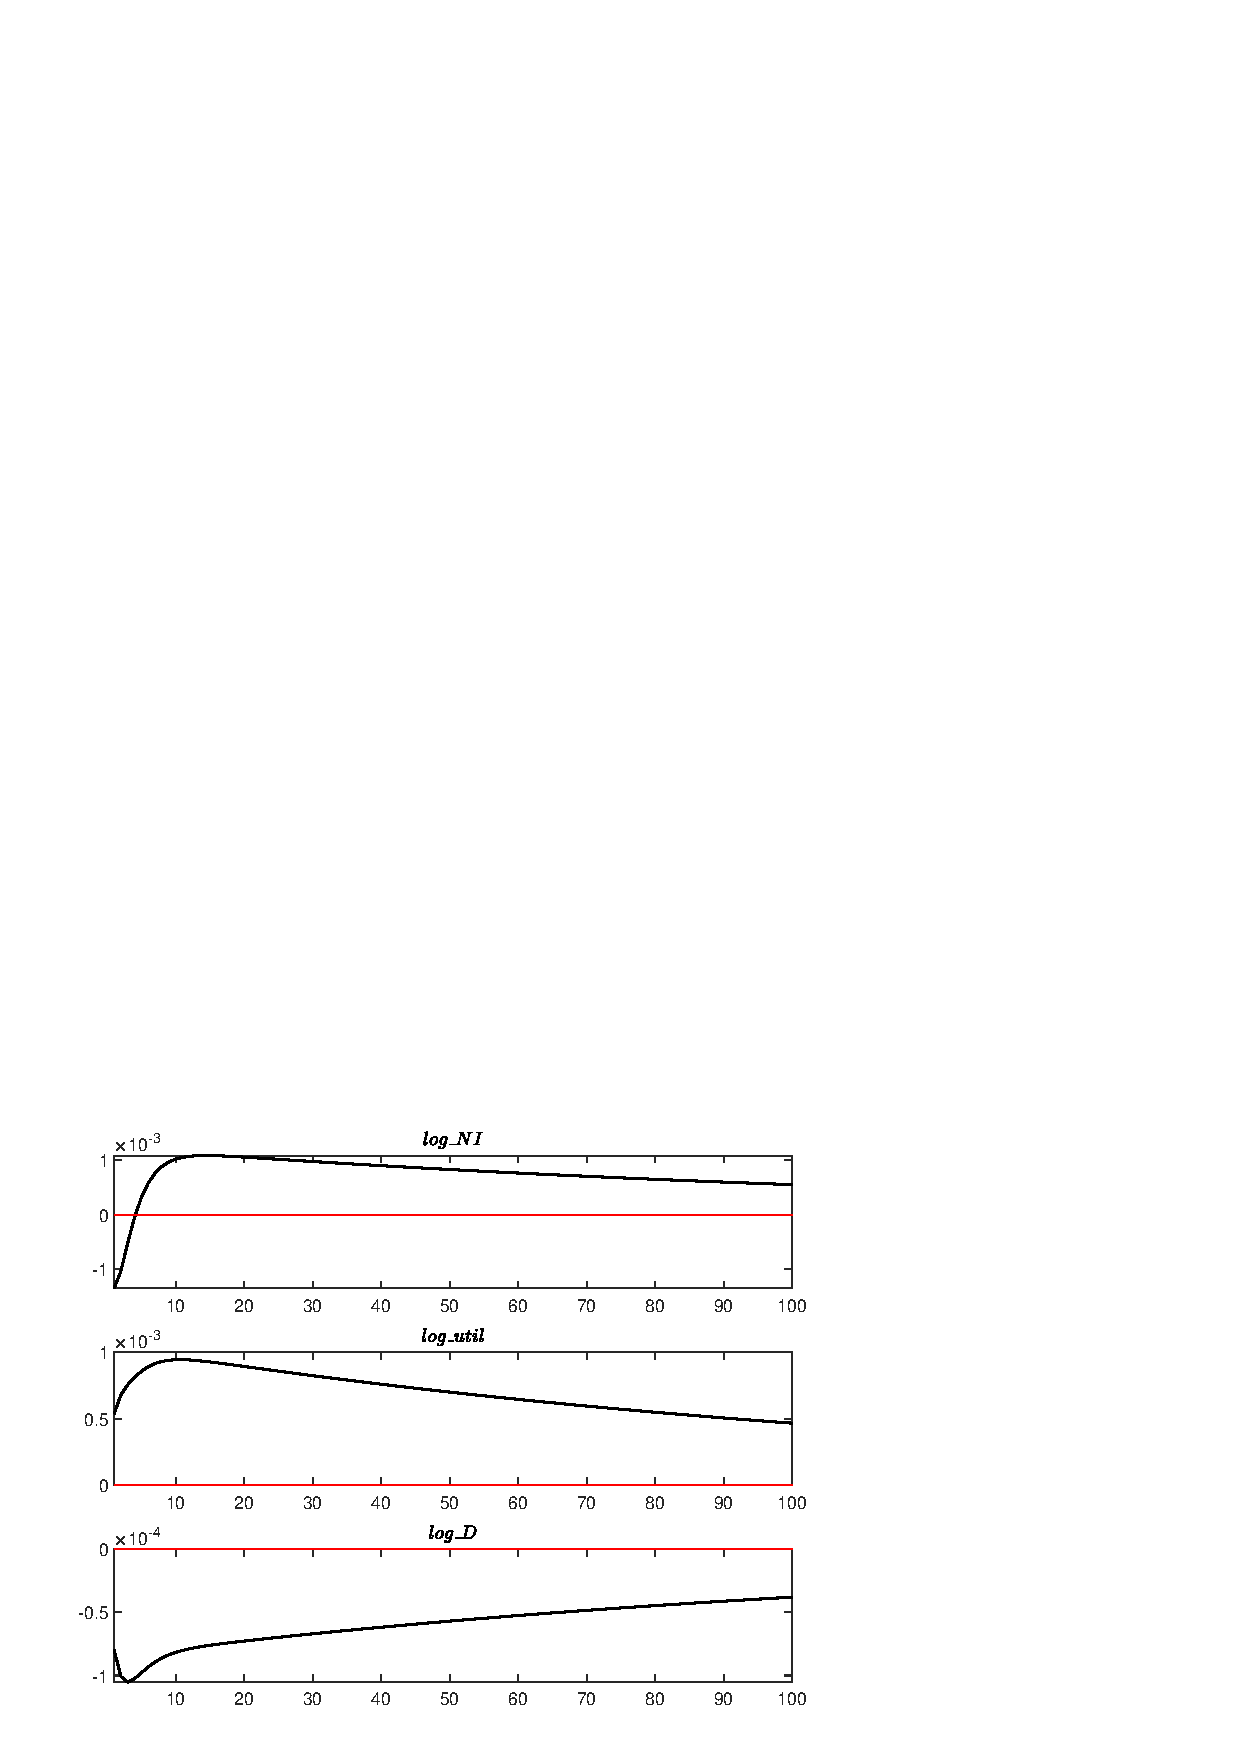
\includegraphics[width=0.80\textwidth]{BRS_growth/graphs/BRS_growth_IRF_e_g3}
\caption{Impulse response functions (orthogonalized shock to ${e_g}$).}\label{Fig:IRF:e_g:3}
\end{figure}
 
\begin{figure}[H]
\centering 
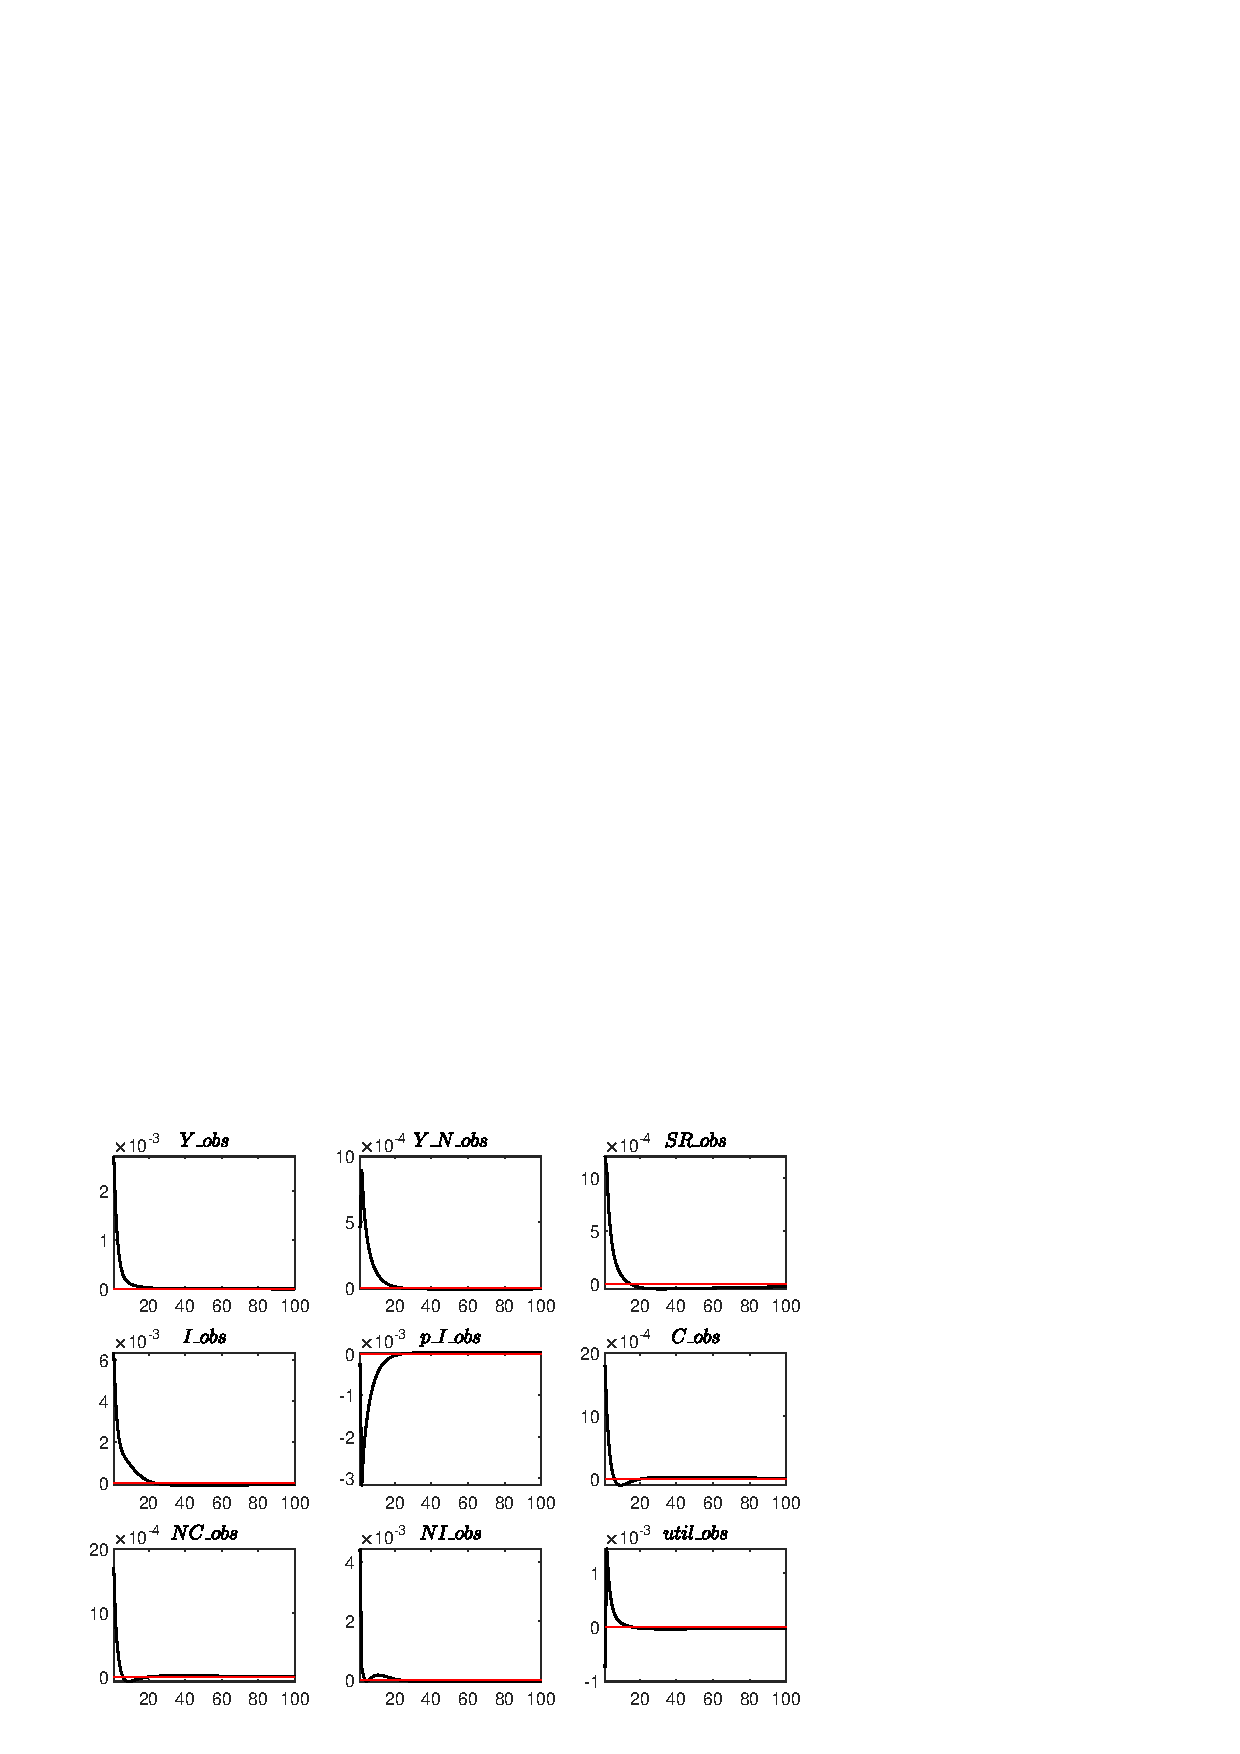
\includegraphics[width=0.80\textwidth]{BRS_growth/graphs/BRS_growth_IRF_e_Z1}
\caption{Impulse response functions (orthogonalized shock to ${e_Z}$).}\label{Fig:IRF:e_Z:1}
\end{figure}
 
\begin{figure}[H]
\centering 
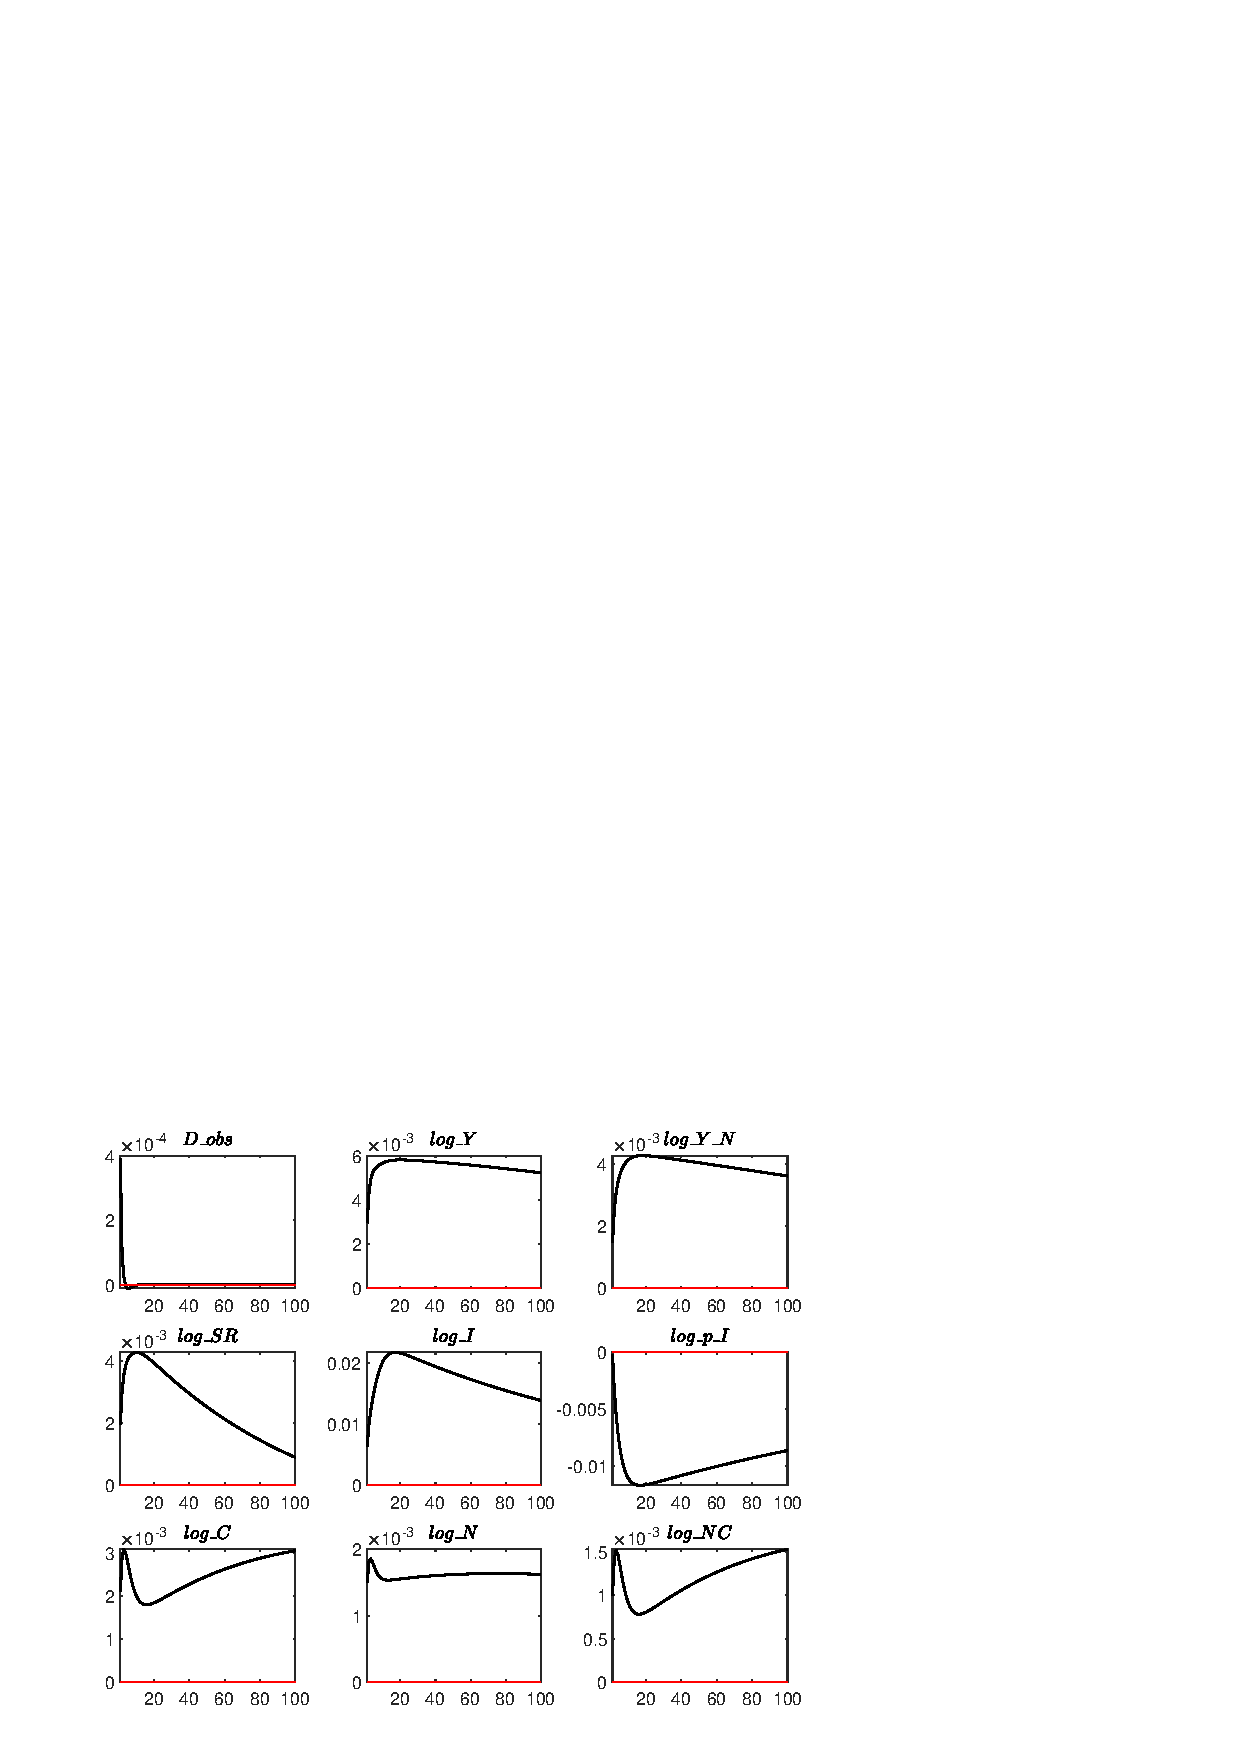
\includegraphics[width=0.80\textwidth]{BRS_growth/graphs/BRS_growth_IRF_e_Z2}
\caption{Impulse response functions (orthogonalized shock to ${e_Z}$).}\label{Fig:IRF:e_Z:2}
\end{figure}
 
\begin{figure}[H]
\centering 
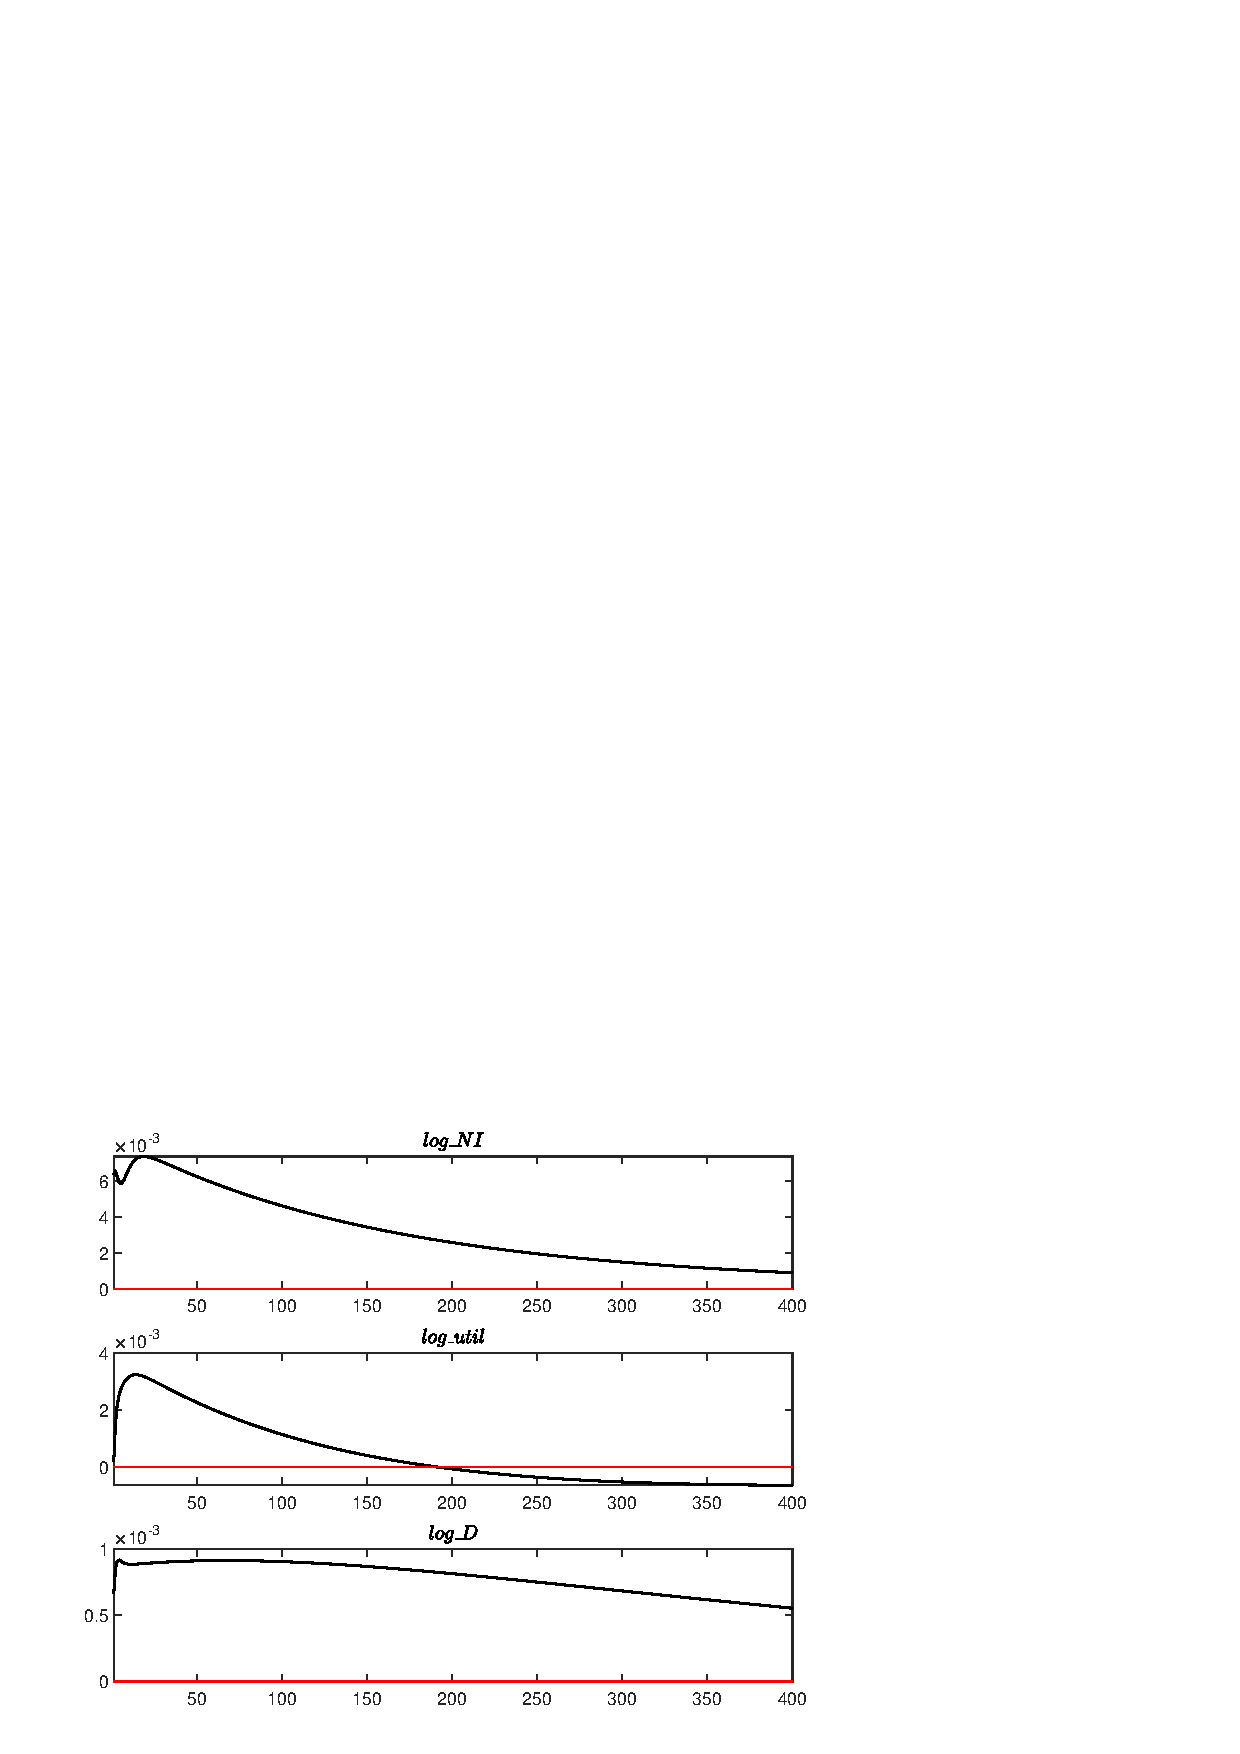
\includegraphics[width=0.80\textwidth]{BRS_growth/graphs/BRS_growth_IRF_e_Z3}
\caption{Impulse response functions (orthogonalized shock to ${e_Z}$).}\label{Fig:IRF:e_Z:3}
\end{figure}
 
\begin{figure}[H]
\centering 
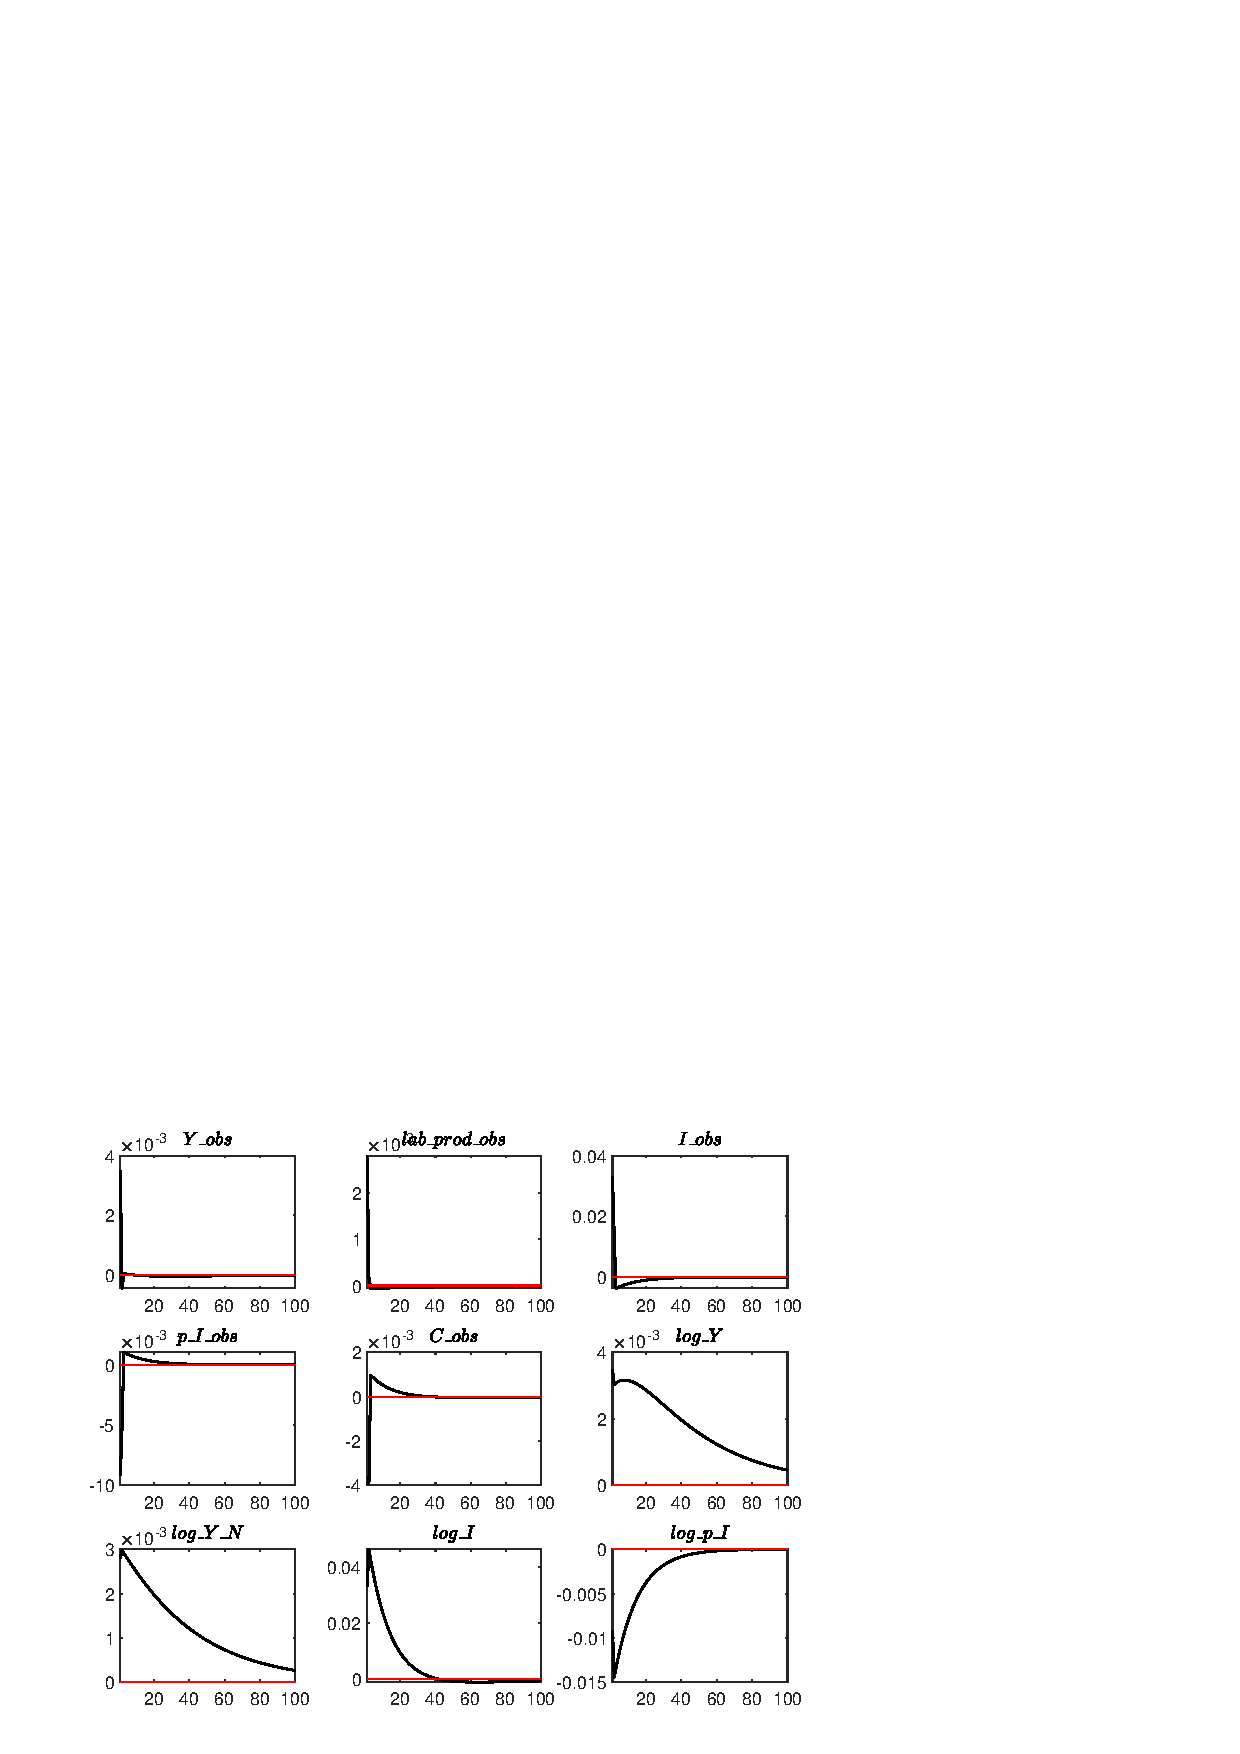
\includegraphics[width=0.80\textwidth]{BRS_growth/graphs/BRS_growth_IRF_e_ZI1}
\caption{Impulse response functions (orthogonalized shock to ${e_{ZI}}$).}\label{Fig:IRF:e_ZI:1}
\end{figure}
 
\begin{figure}[H]
\centering 
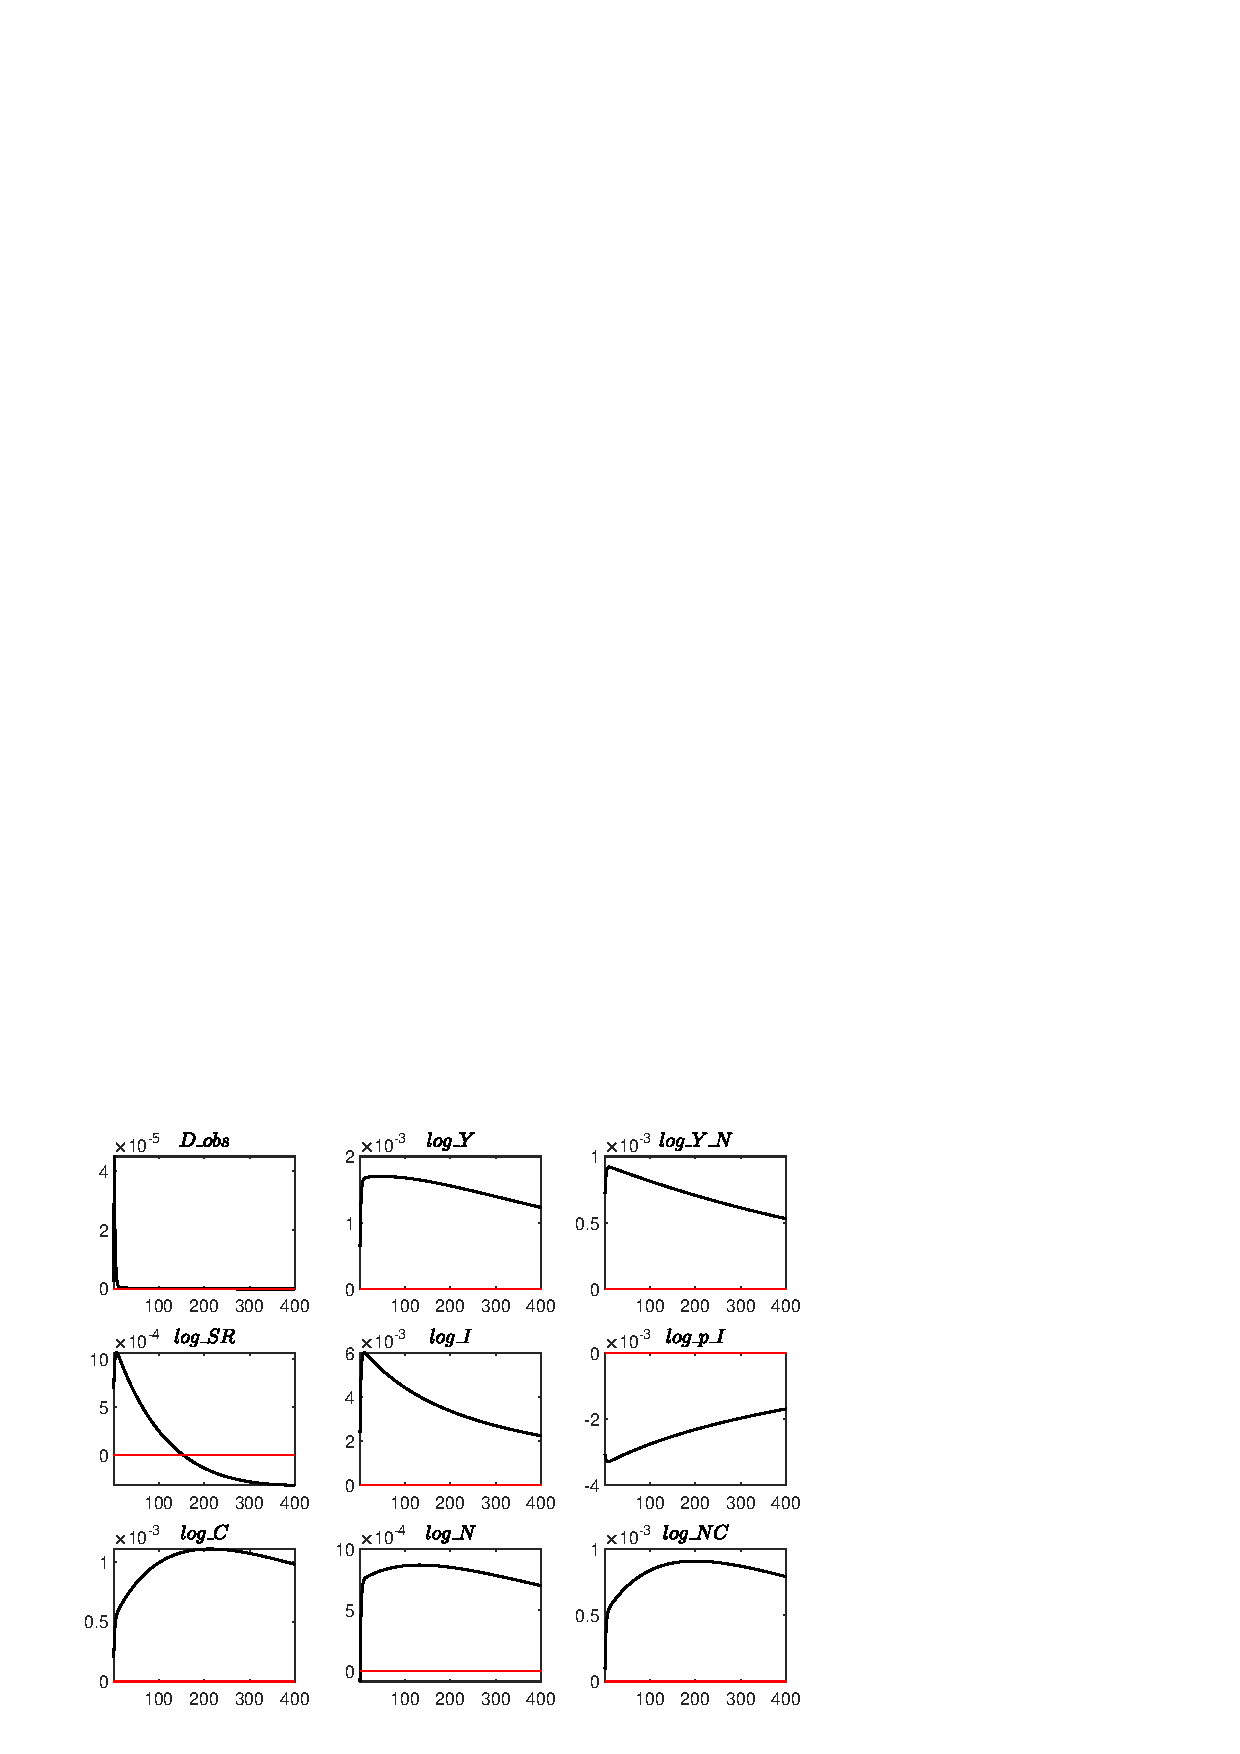
\includegraphics[width=0.80\textwidth]{BRS_growth/graphs/BRS_growth_IRF_e_ZI2}
\caption{Impulse response functions (orthogonalized shock to ${e_{ZI}}$).}\label{Fig:IRF:e_ZI:2}
\end{figure}
 
\begin{figure}[H]
\centering 
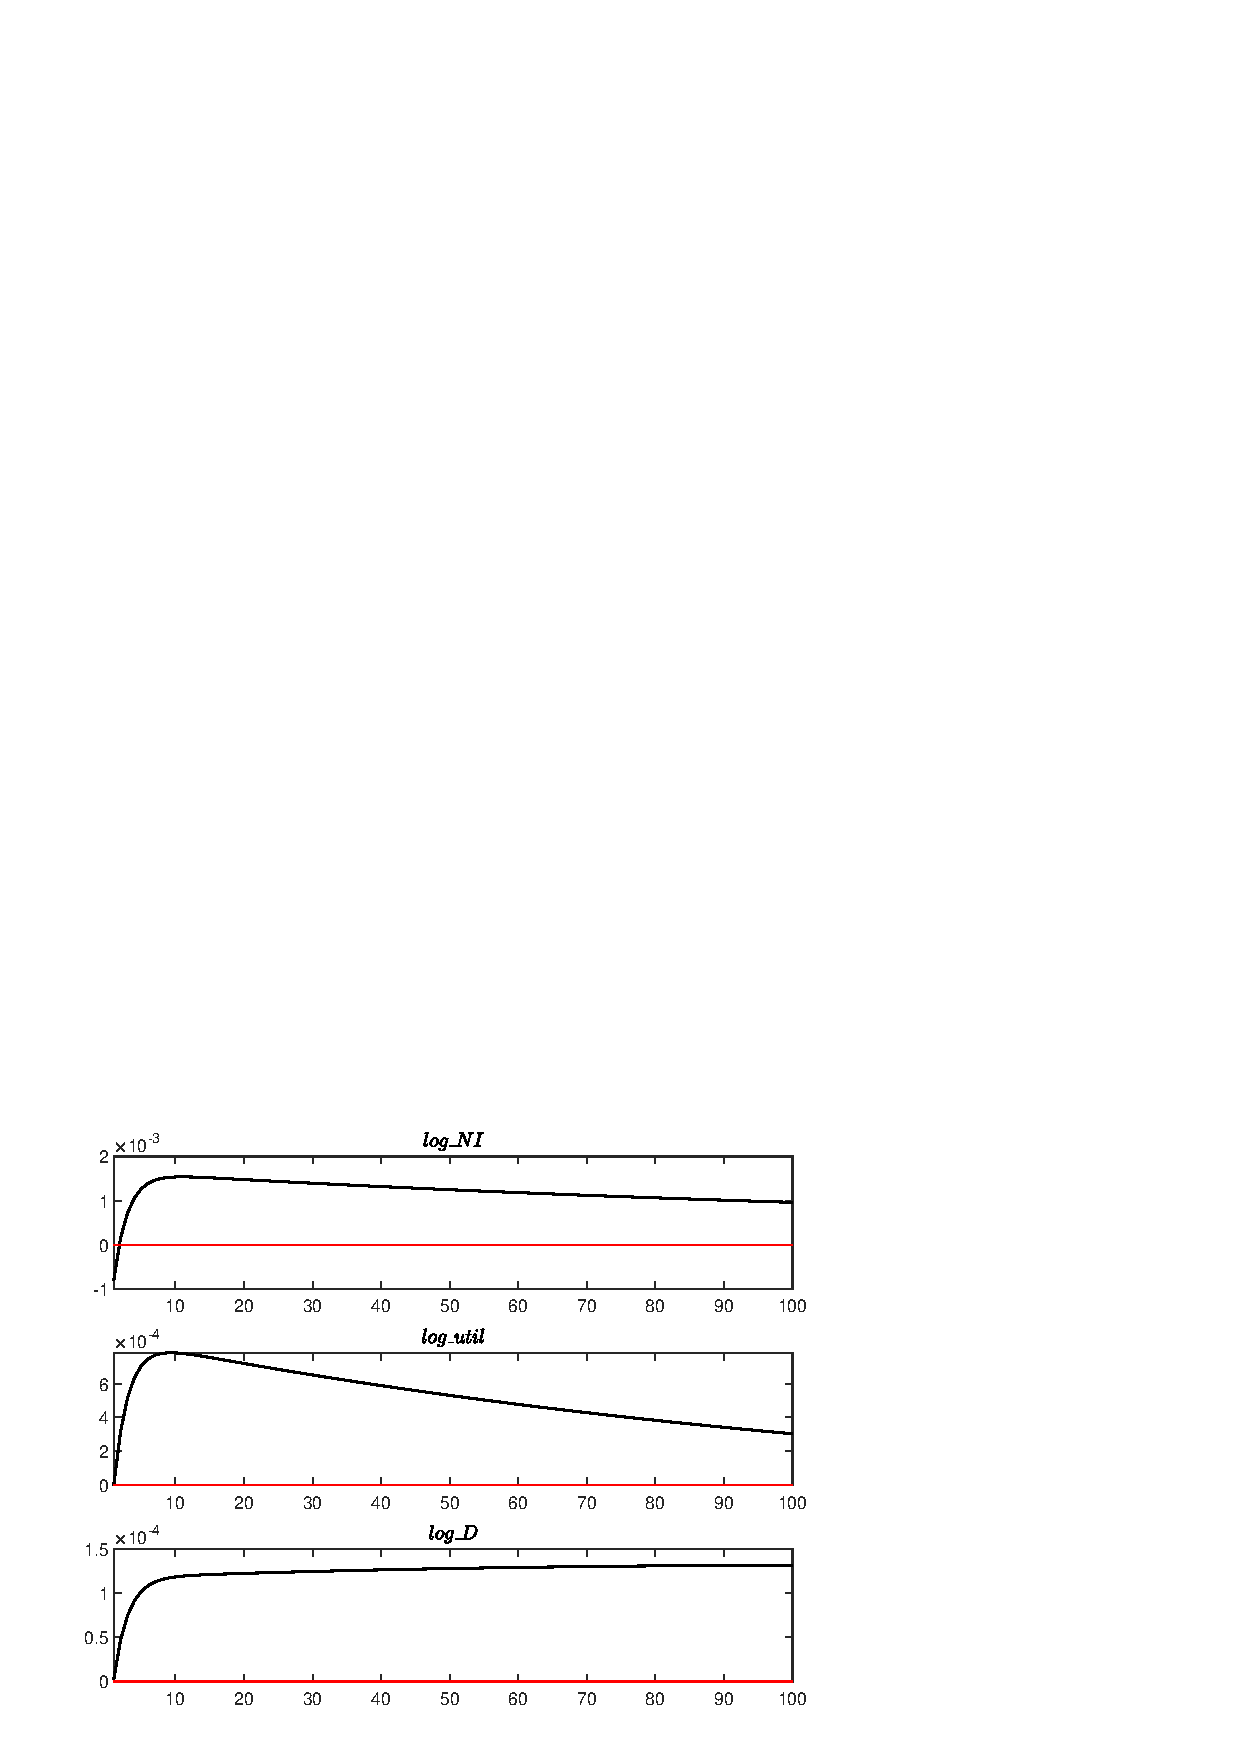
\includegraphics[width=0.80\textwidth]{BRS_growth/graphs/BRS_growth_IRF_e_ZI3}
\caption{Impulse response functions (orthogonalized shock to ${e_{ZI}}$).}\label{Fig:IRF:e_ZI:3}
\end{figure}
 
\begin{figure}[H]
\centering 
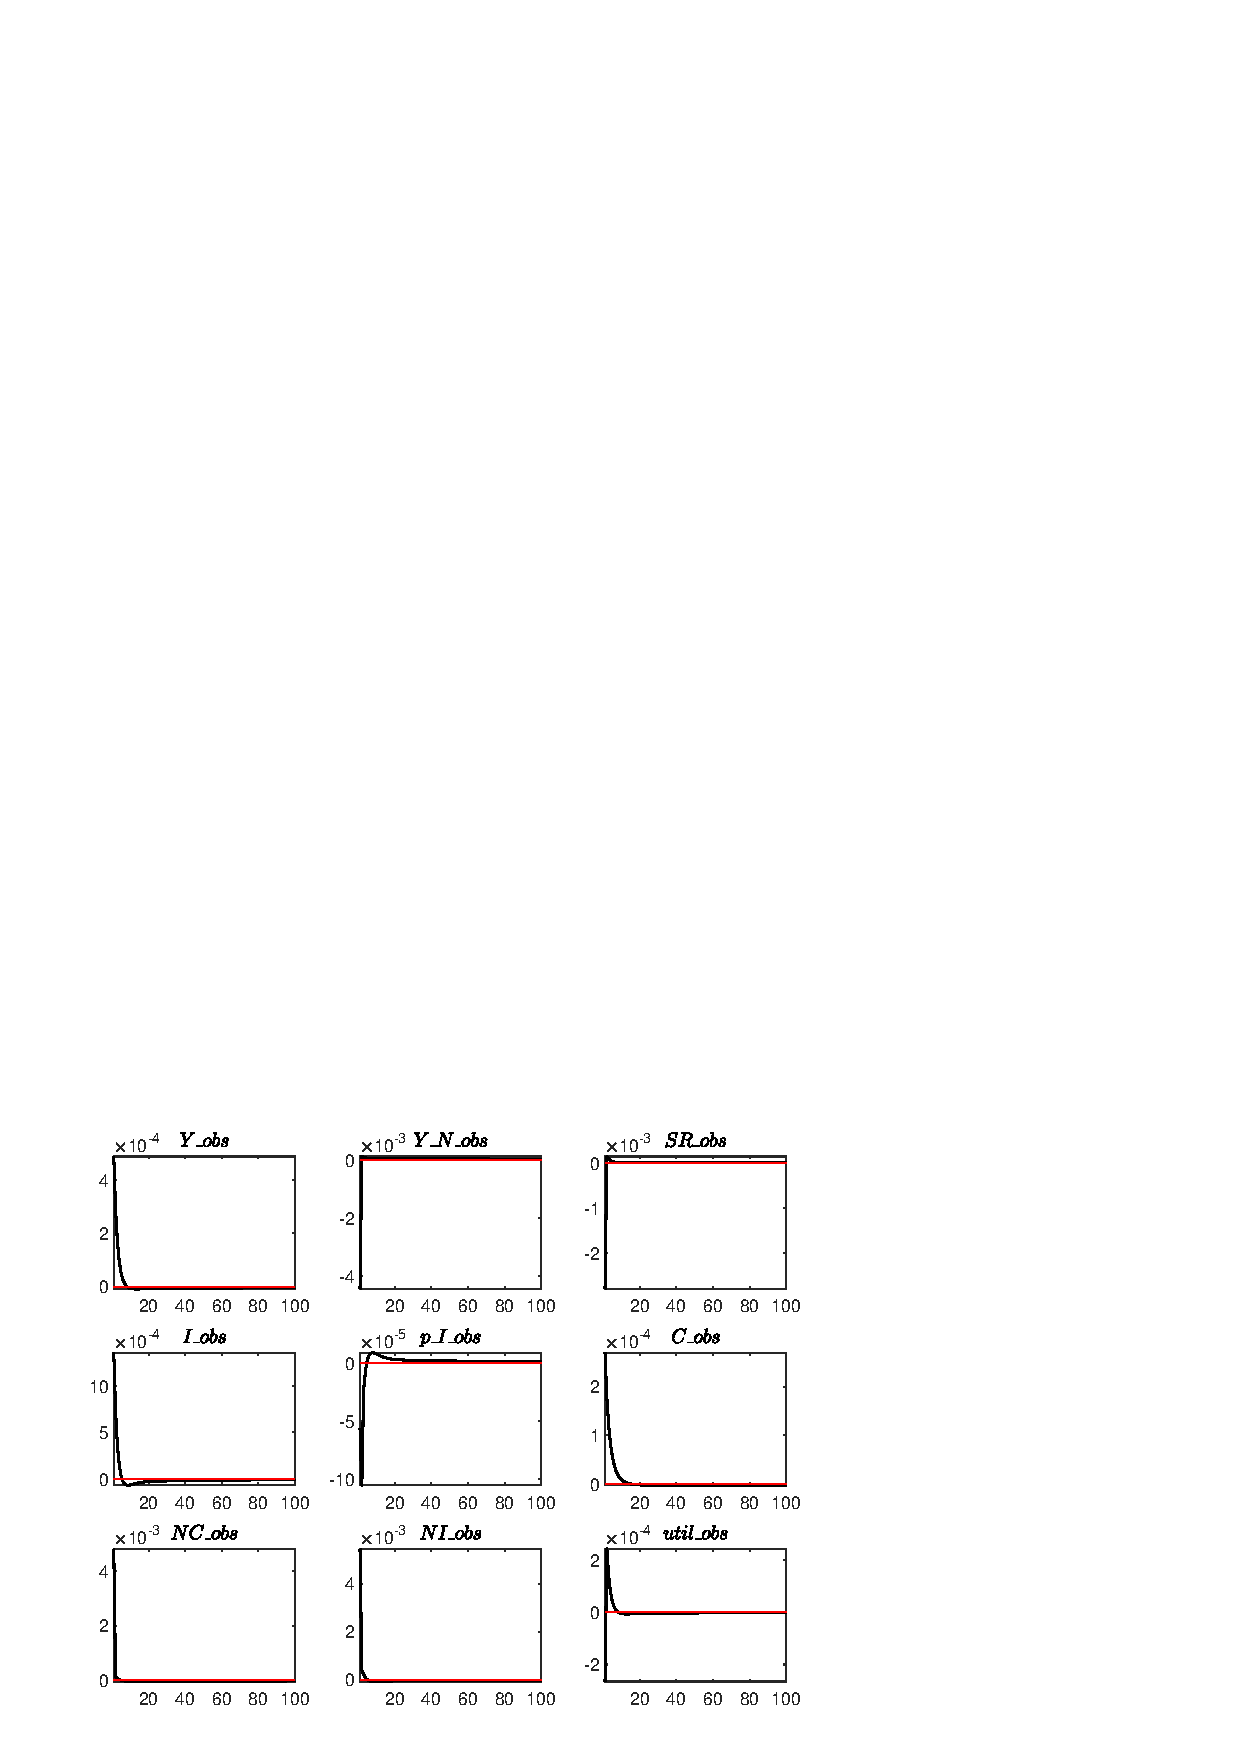
\includegraphics[width=0.80\textwidth]{BRS_growth/graphs/BRS_growth_IRF_e_N1}
\caption{Impulse response functions (orthogonalized shock to ${e_N}$).}\label{Fig:IRF:e_N:1}
\end{figure}
 
\begin{figure}[H]
\centering 
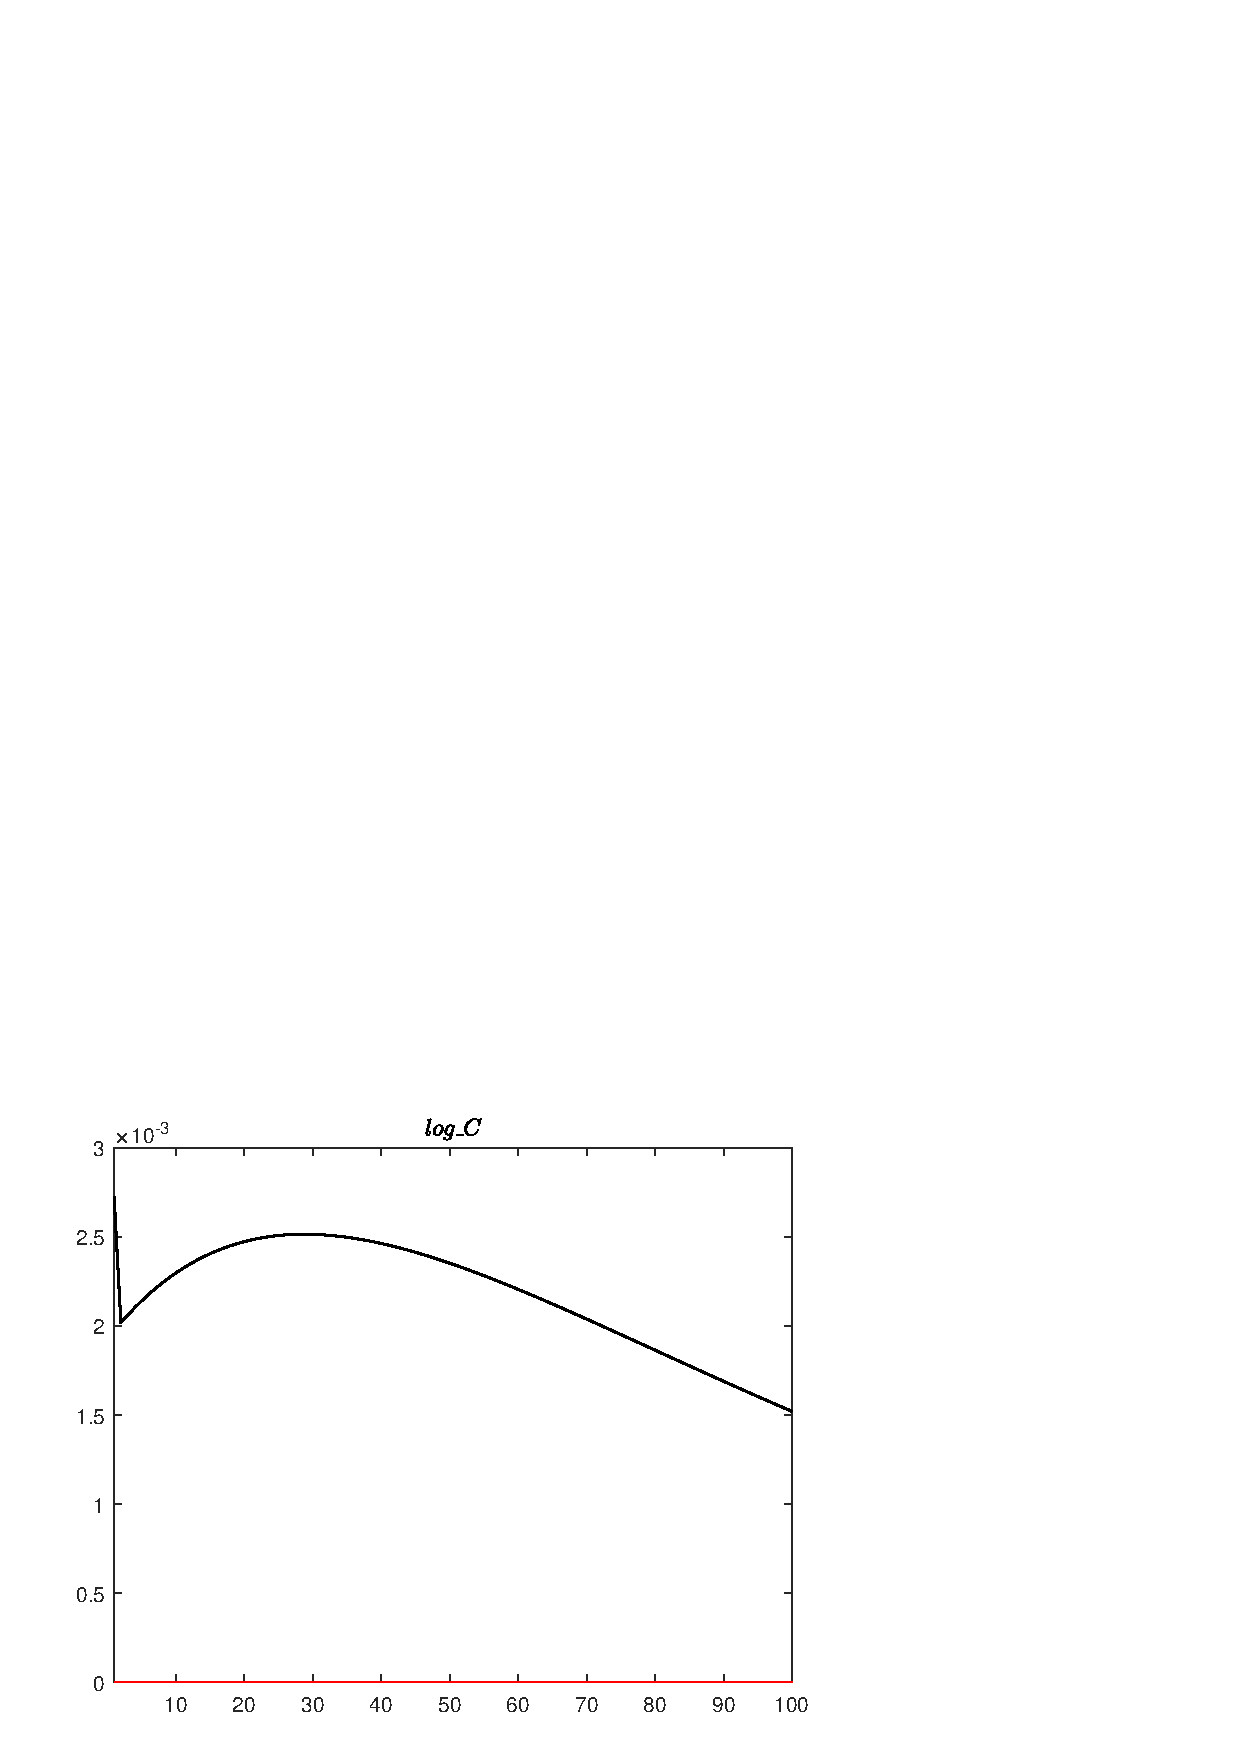
\includegraphics[width=0.80\textwidth]{BRS_growth/graphs/BRS_growth_IRF_e_N2}
\caption{Impulse response functions (orthogonalized shock to ${e_N}$).}\label{Fig:IRF:e_N:2}
\end{figure}
 
\begin{figure}[H]
\centering 
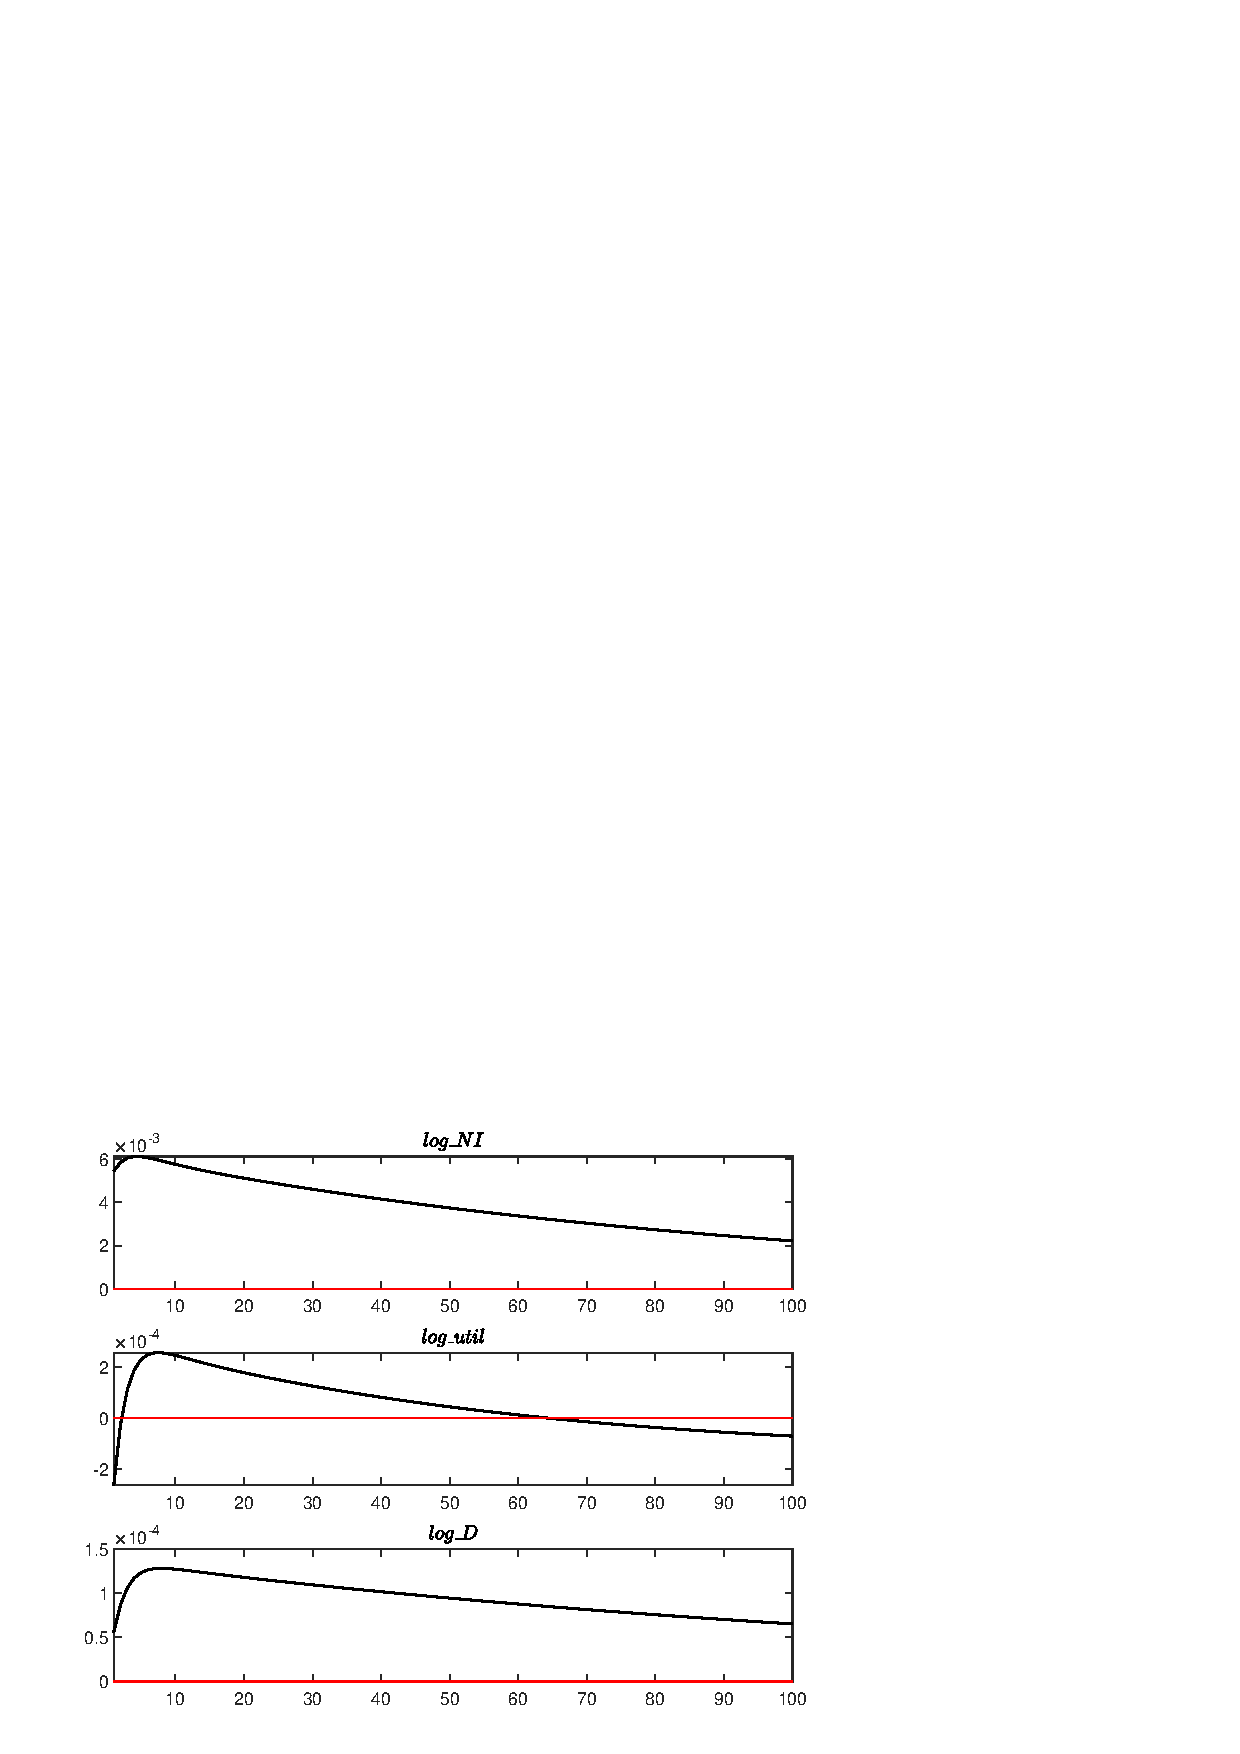
\includegraphics[width=0.80\textwidth]{BRS_growth/graphs/BRS_growth_IRF_e_N3}
\caption{Impulse response functions (orthogonalized shock to ${e_N}$).}\label{Fig:IRF:e_N:3}
\end{figure}
 
\begin{figure}[H]
\centering 
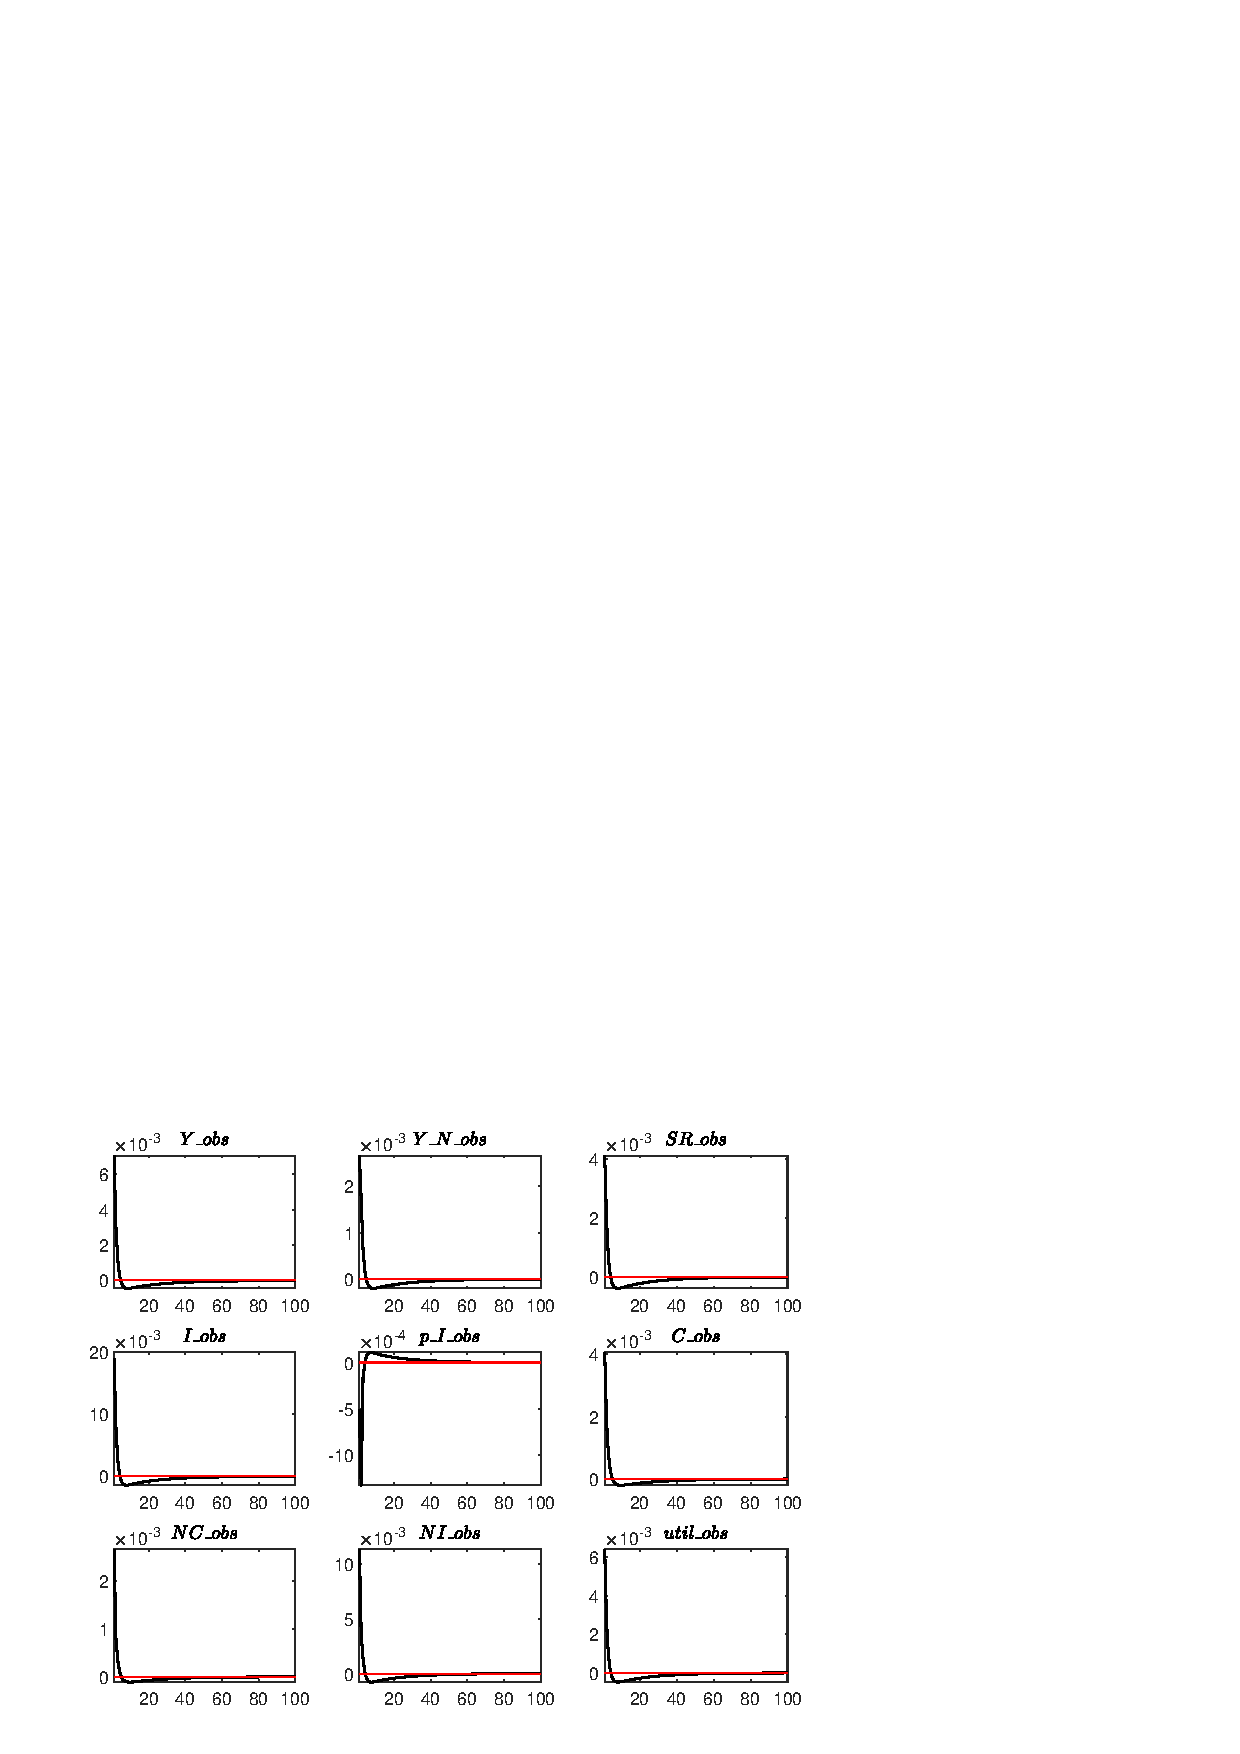
\includegraphics[width=0.80\textwidth]{BRS_growth/graphs/BRS_growth_IRF_e_D1}
\caption{Impulse response functions (orthogonalized shock to ${e_D}$).}\label{Fig:IRF:e_D:1}
\end{figure}
 
\begin{figure}[H]
\centering 
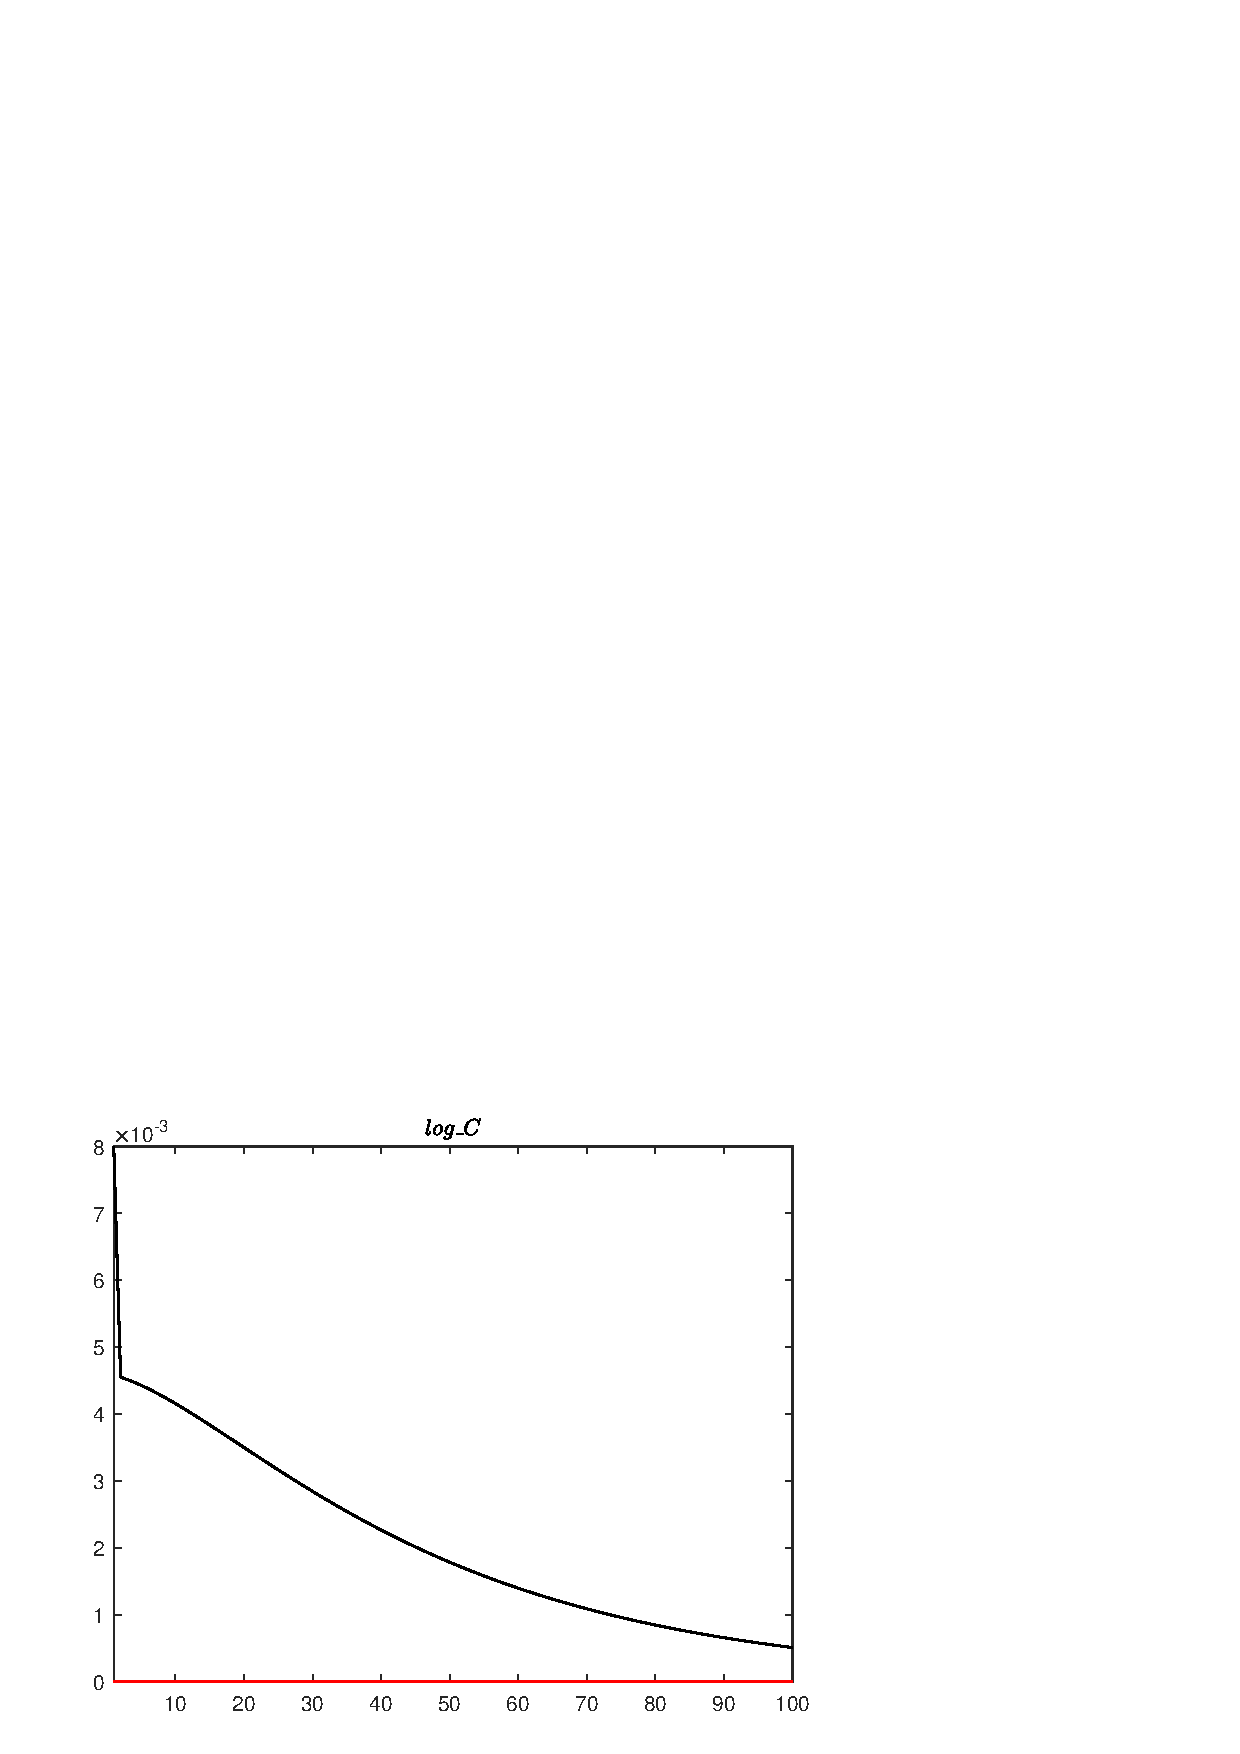
\includegraphics[width=0.80\textwidth]{BRS_growth/graphs/BRS_growth_IRF_e_D2}
\caption{Impulse response functions (orthogonalized shock to ${e_D}$).}\label{Fig:IRF:e_D:2}
\end{figure}
 
\begin{figure}[H]
\centering 
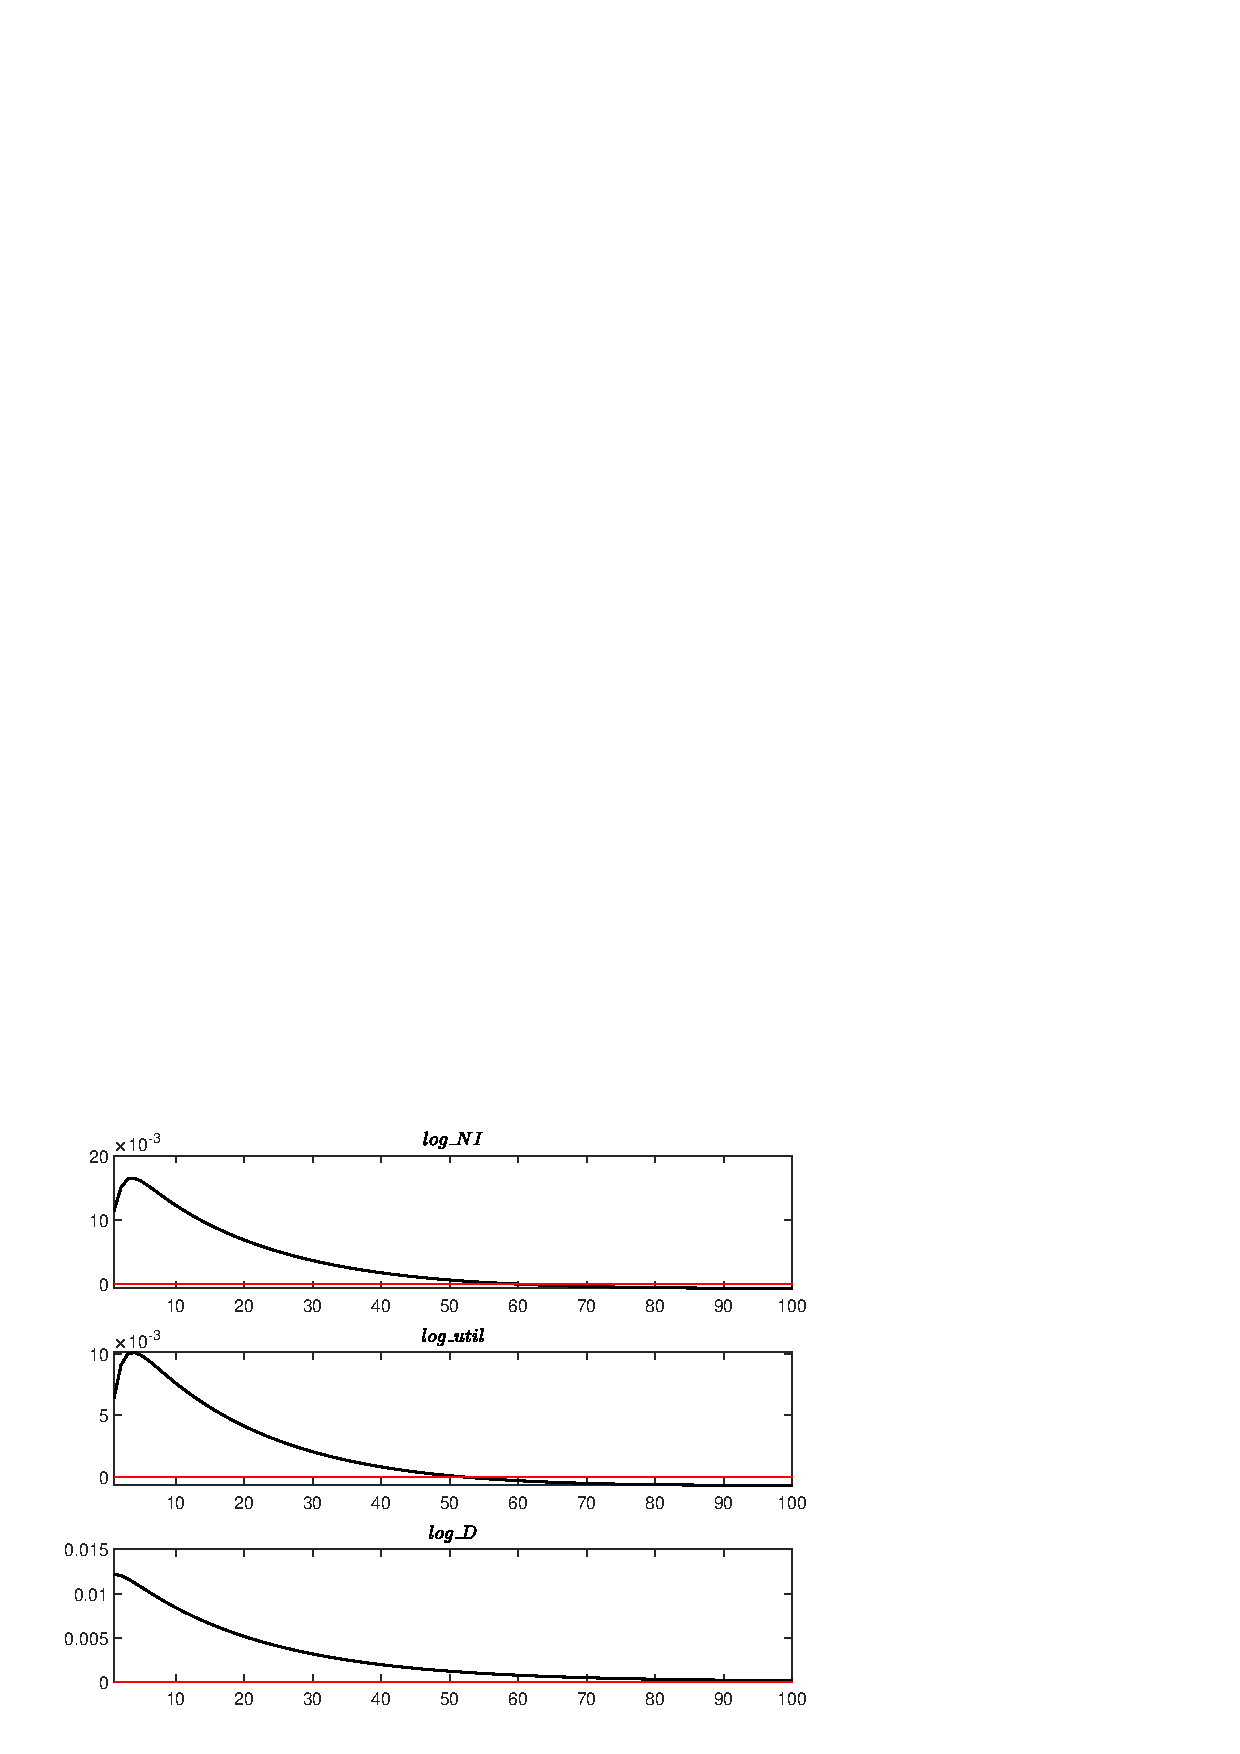
\includegraphics[width=0.80\textwidth]{BRS_growth/graphs/BRS_growth_IRF_e_D3}
\caption{Impulse response functions (orthogonalized shock to ${e_D}$).}\label{Fig:IRF:e_D:3}
\end{figure}
 
\begin{figure}[H]
\centering 
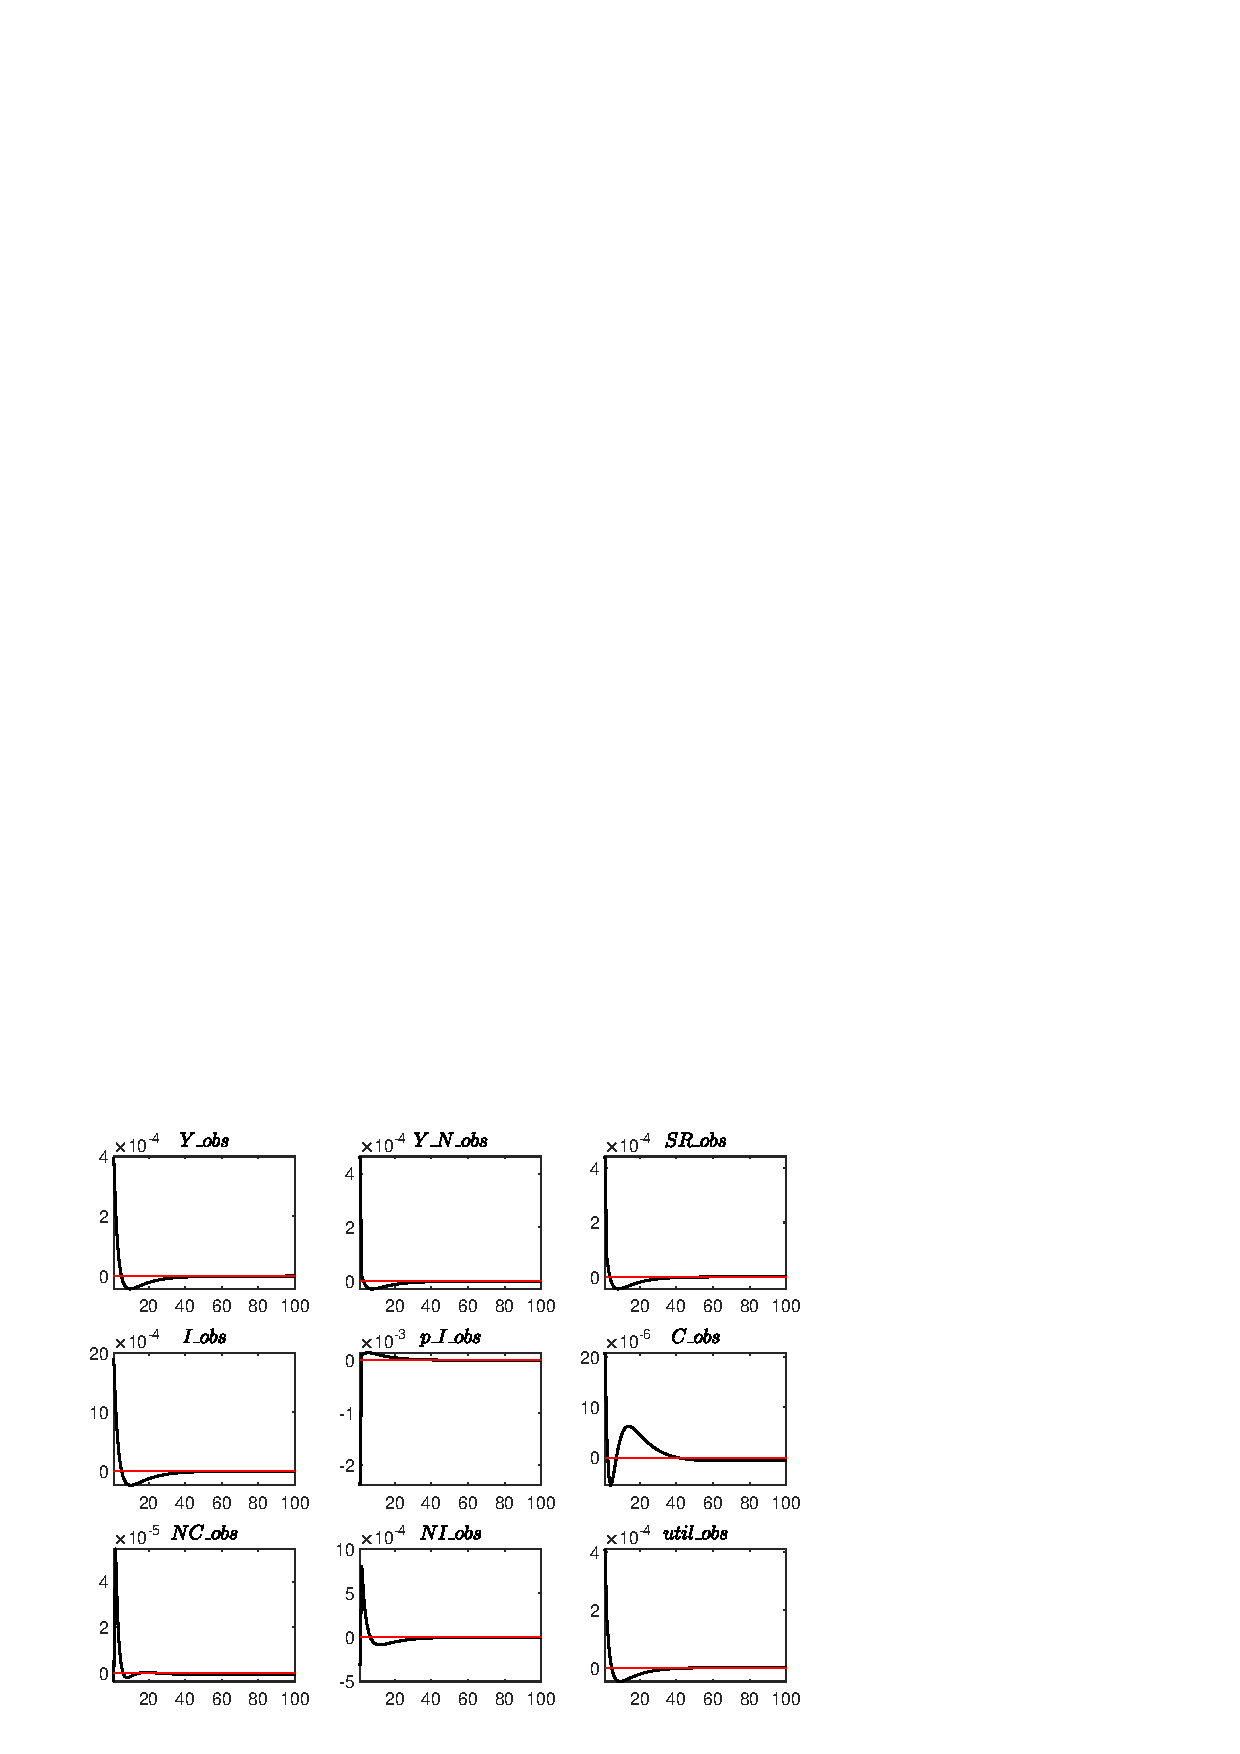
\includegraphics[width=0.80\textwidth]{BRS_growth/graphs/BRS_growth_IRF_e_DI1}
\caption{Impulse response functions (orthogonalized shock to ${e_DI}$).}\label{Fig:IRF:e_DI:1}
\end{figure}
 
\begin{figure}[H]
\centering 
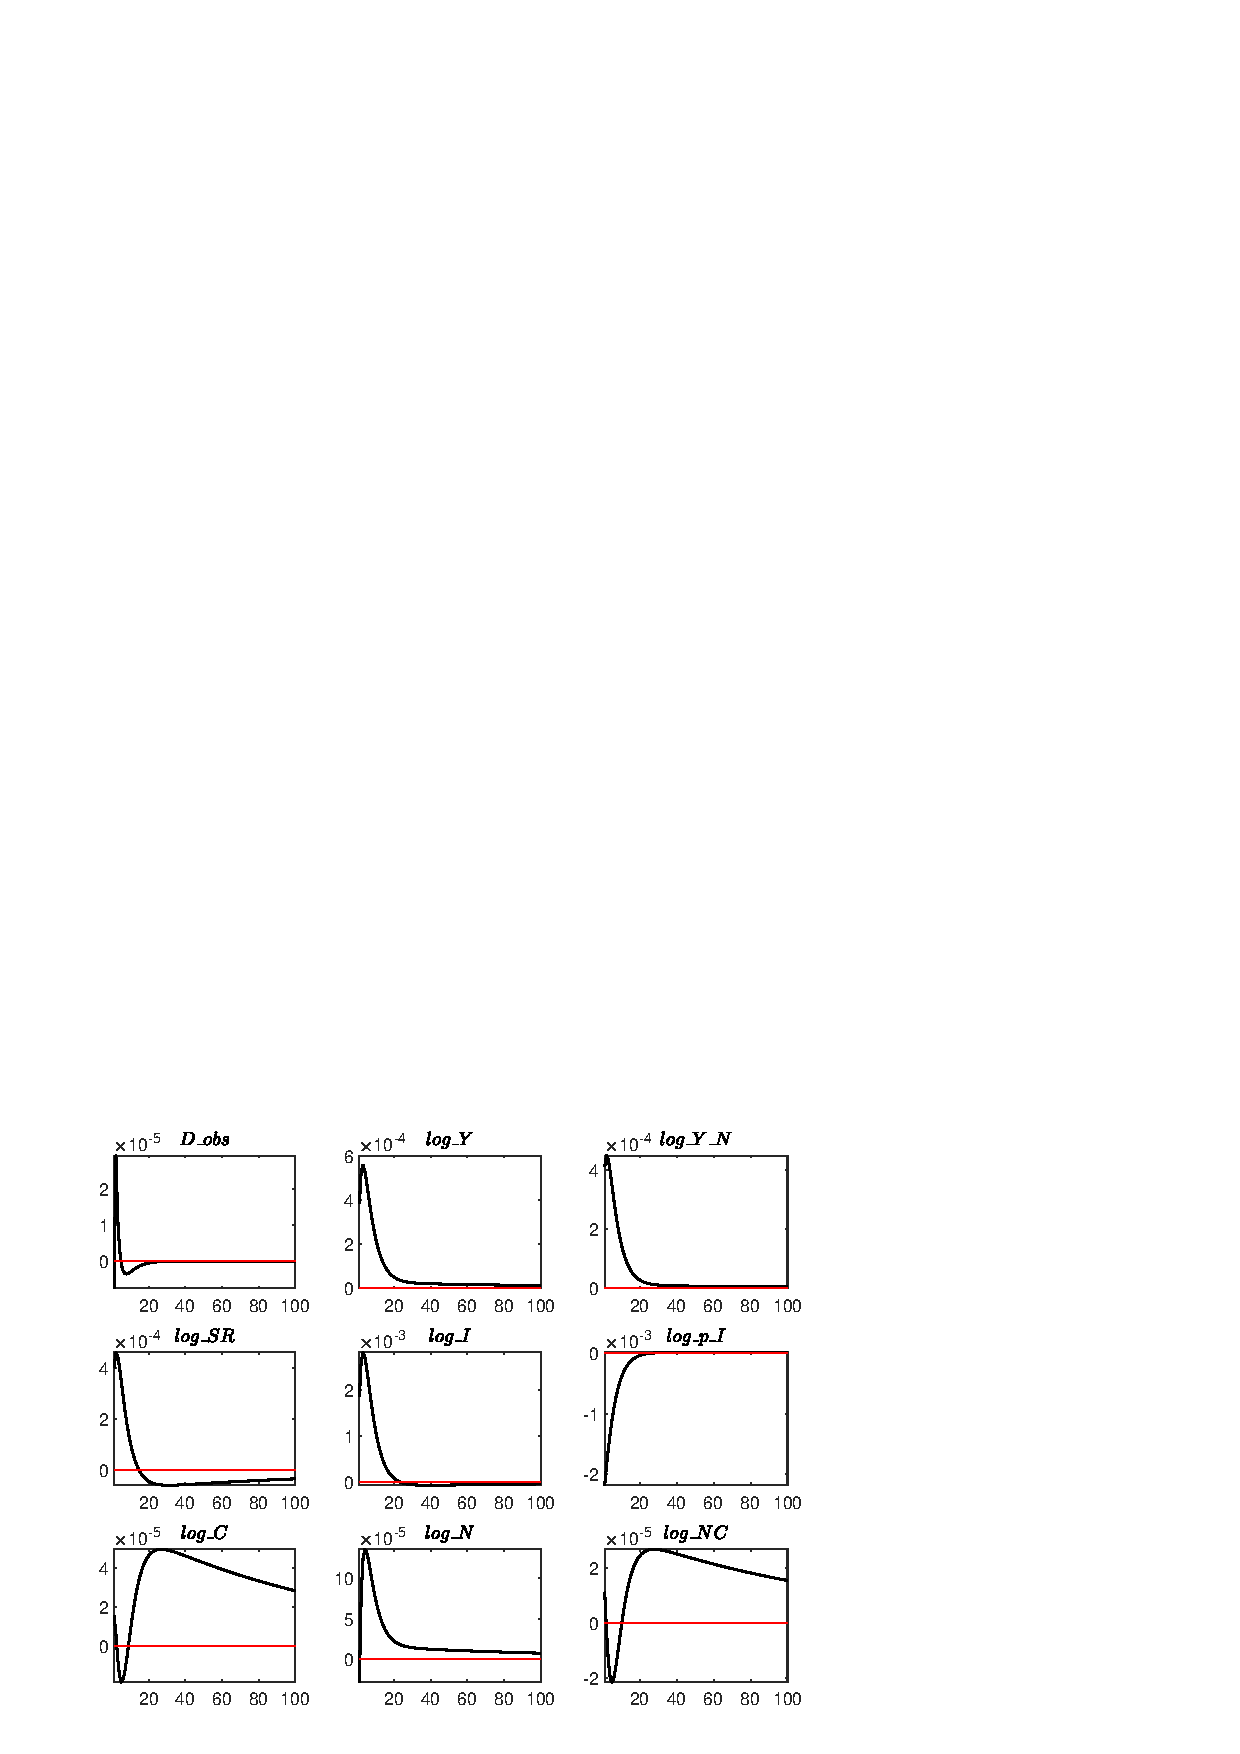
\includegraphics[width=0.80\textwidth]{BRS_growth/graphs/BRS_growth_IRF_e_DI2}
\caption{Impulse response functions (orthogonalized shock to ${e_DI}$).}\label{Fig:IRF:e_DI:2}
\end{figure}
 
\begin{figure}[H]
\centering 
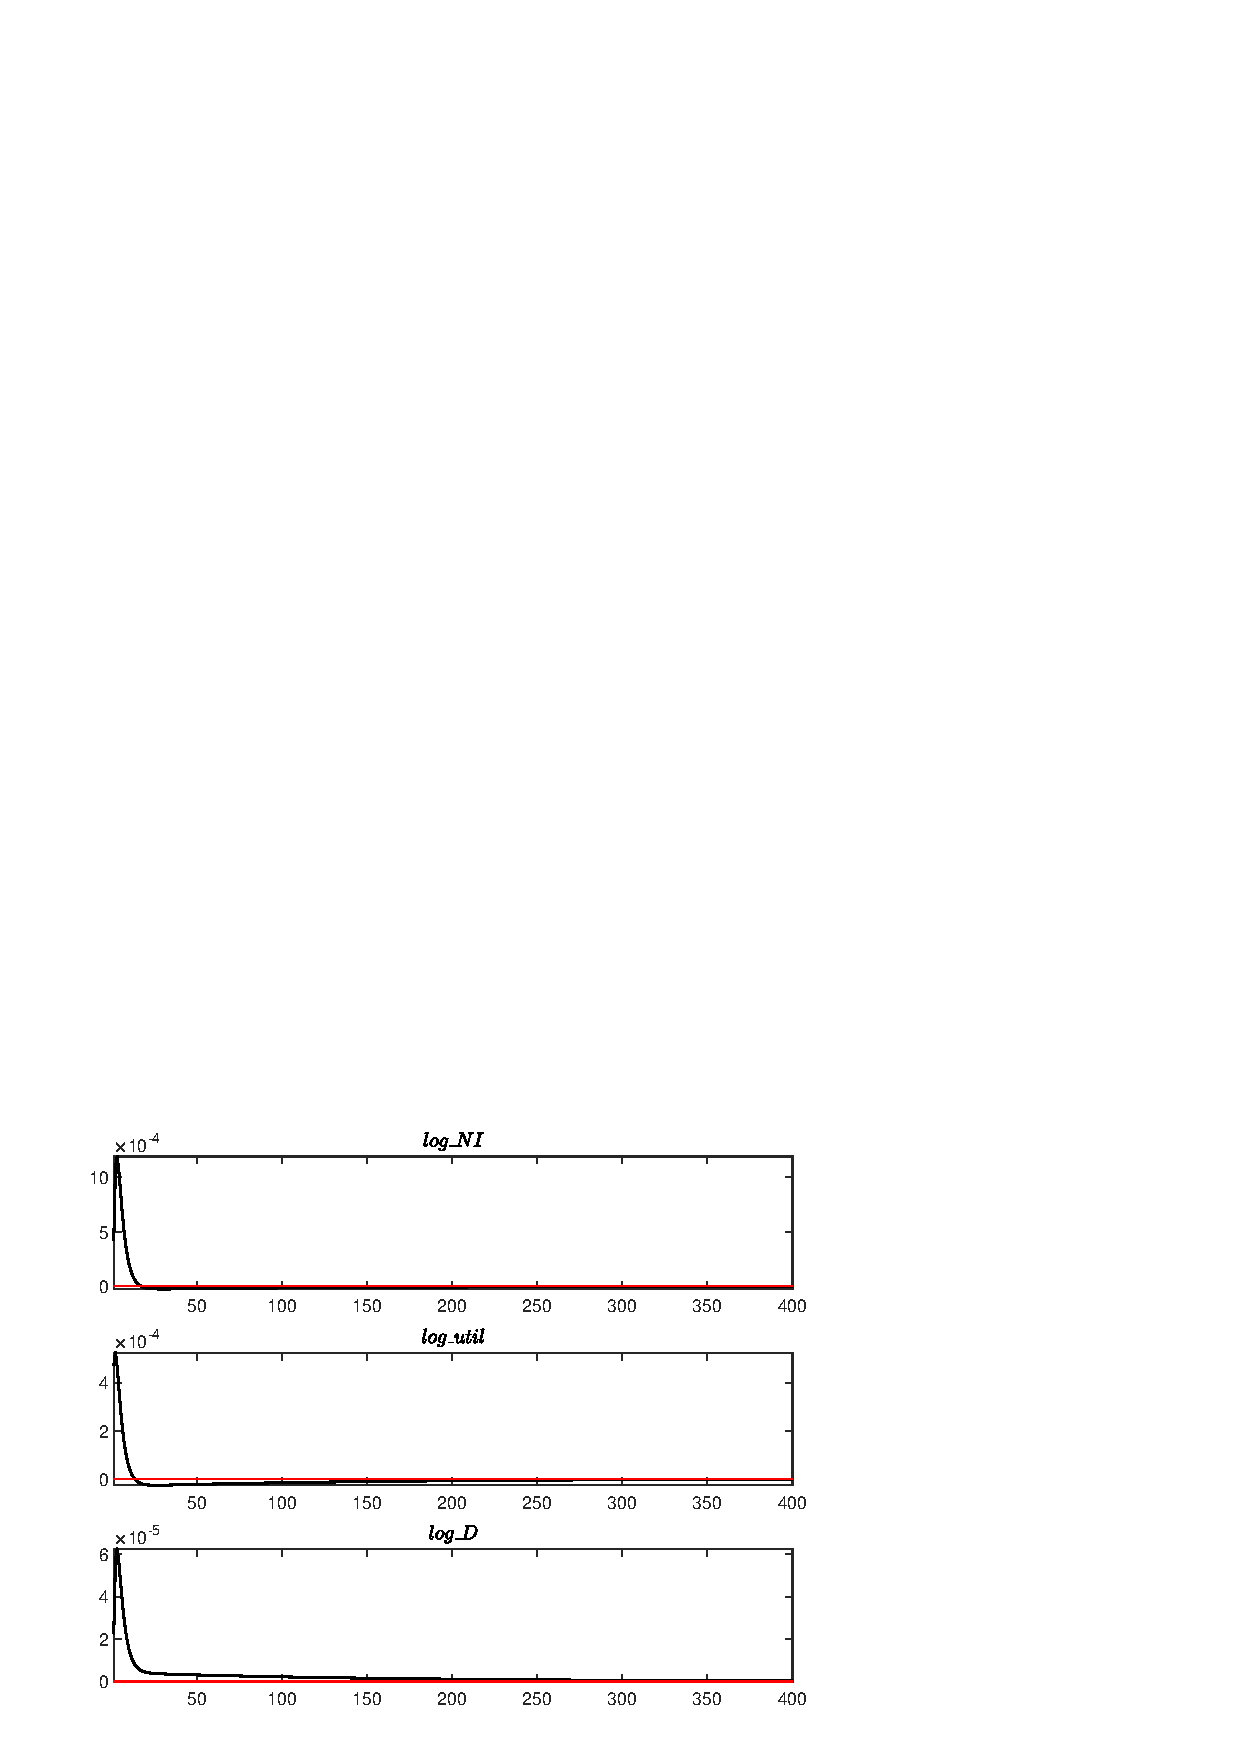
\includegraphics[width=0.80\textwidth]{BRS_growth/graphs/BRS_growth_IRF_e_DI3}
\caption{Impulse response functions (orthogonalized shock to ${e_DI}$).}\label{Fig:IRF:e_DI:3}
\end{figure}
 
\begin{figure}[H]
\centering 
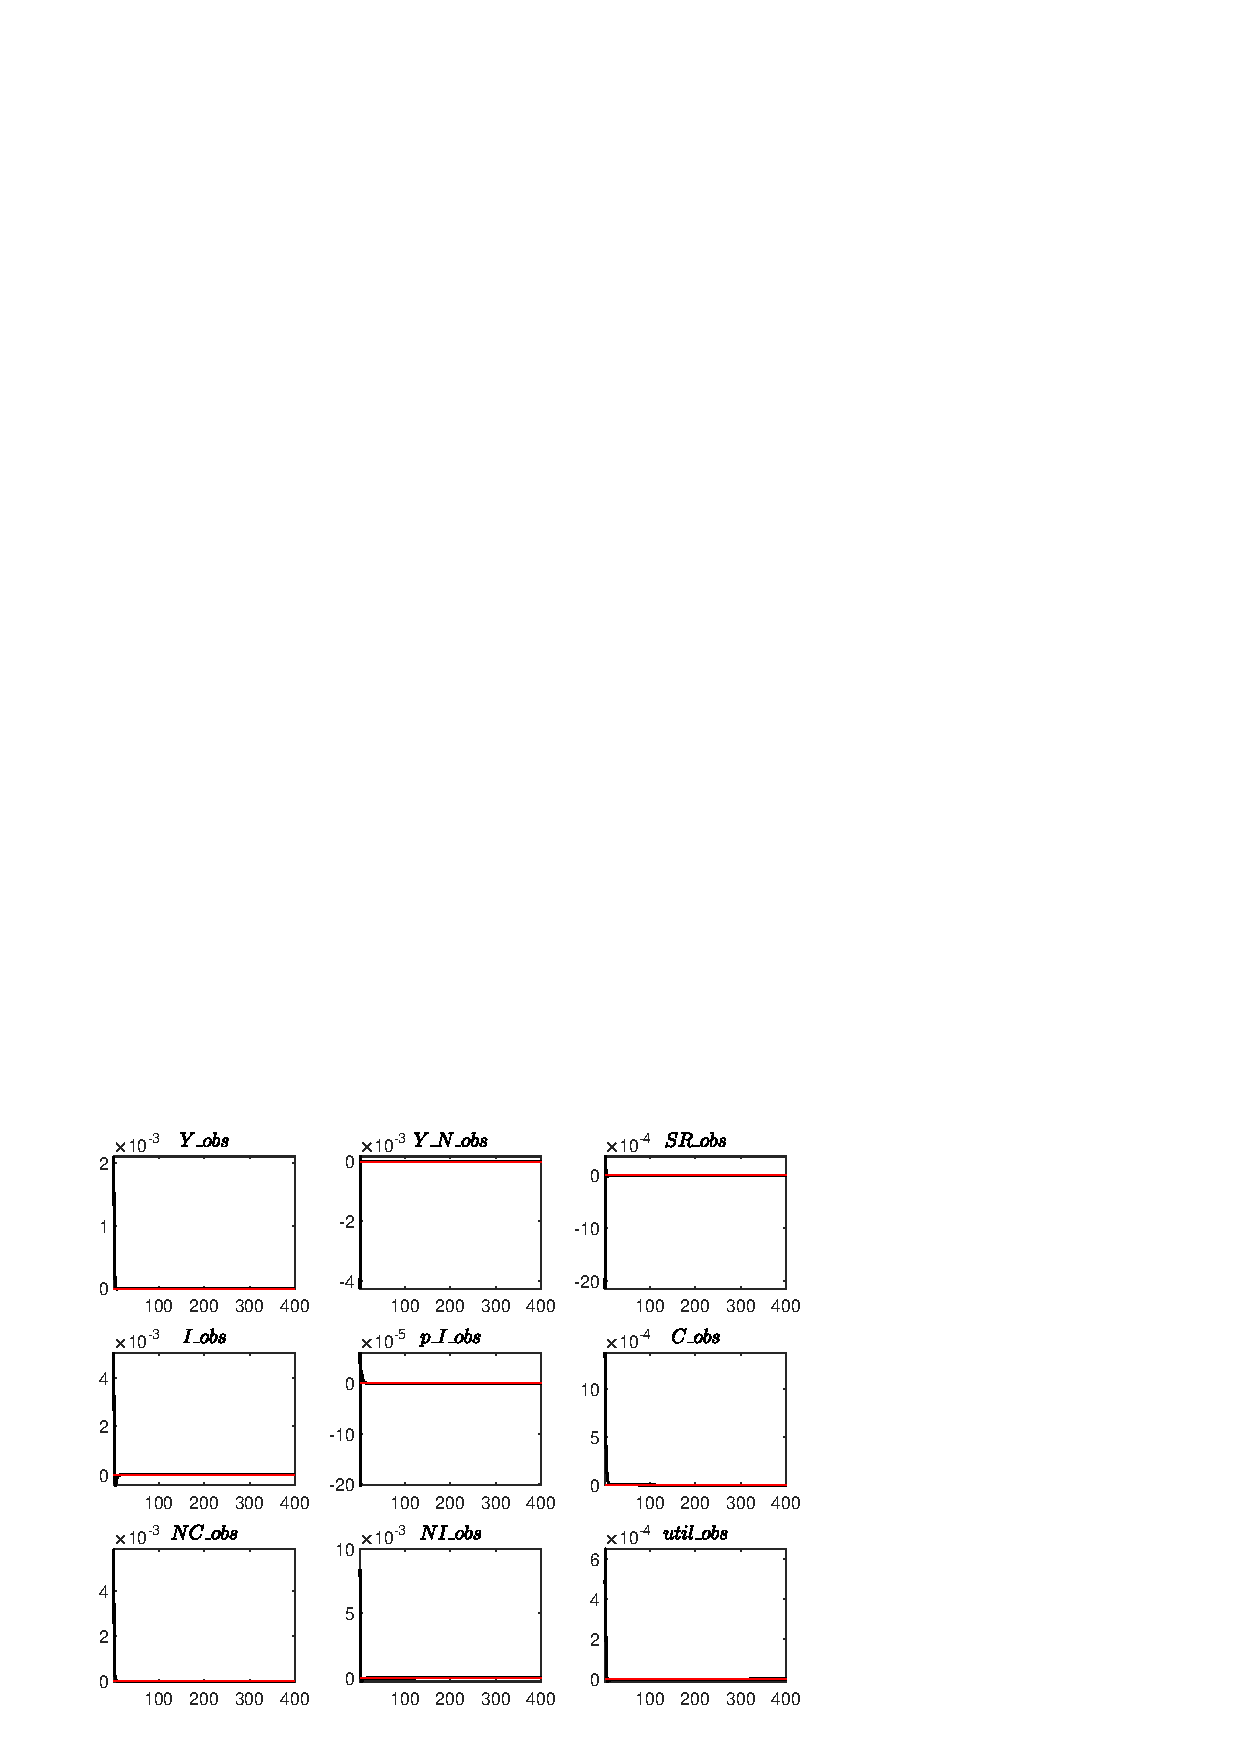
\includegraphics[width=0.80\textwidth]{BRS_growth/graphs/BRS_growth_IRF_e_C1}
\caption{Impulse response functions (orthogonalized shock to ${e_C}$).}\label{Fig:IRF:e_C:1}
\end{figure}
 
\begin{figure}[H]
\centering 
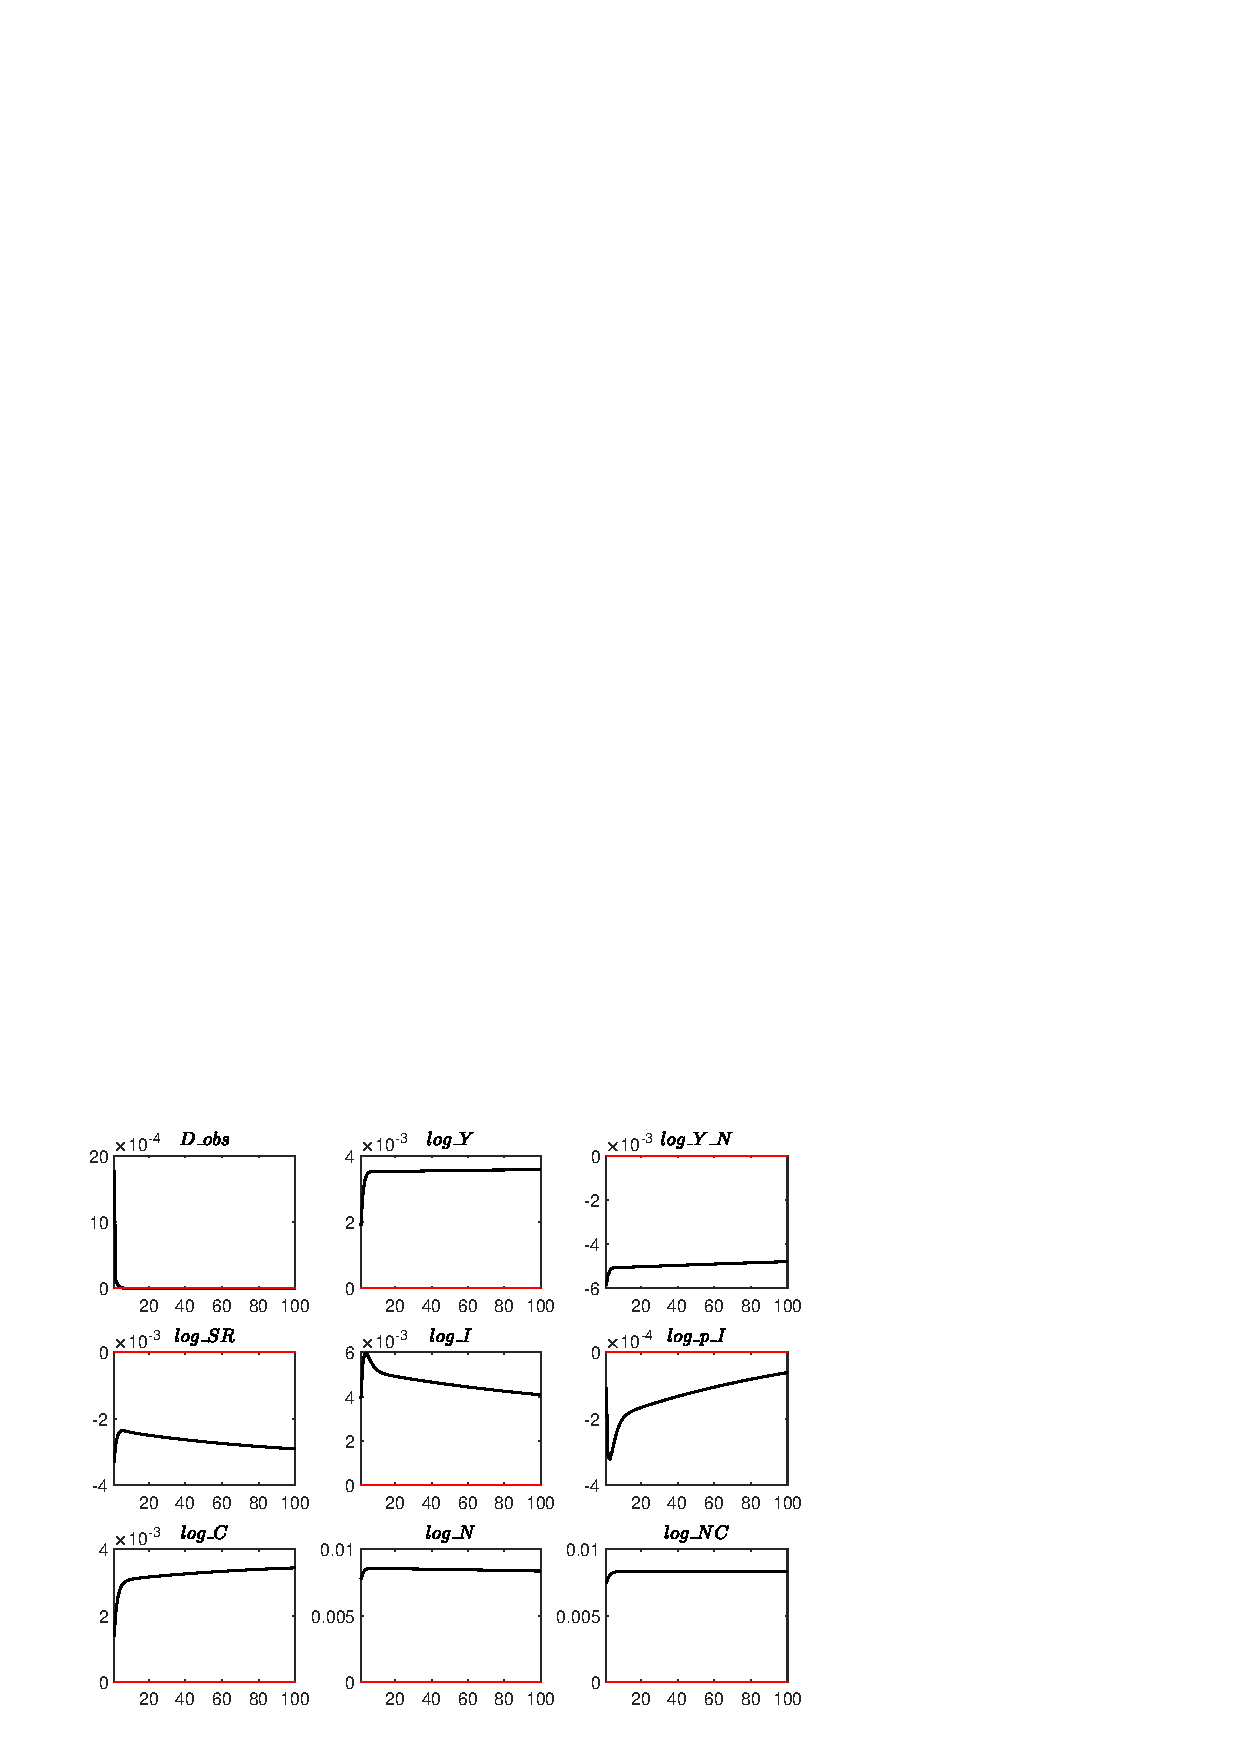
\includegraphics[width=0.80\textwidth]{BRS_growth/graphs/BRS_growth_IRF_e_C2}
\caption{Impulse response functions (orthogonalized shock to ${e_C}$).}\label{Fig:IRF:e_C:2}
\end{figure}
 
\begin{figure}[H]
\centering 
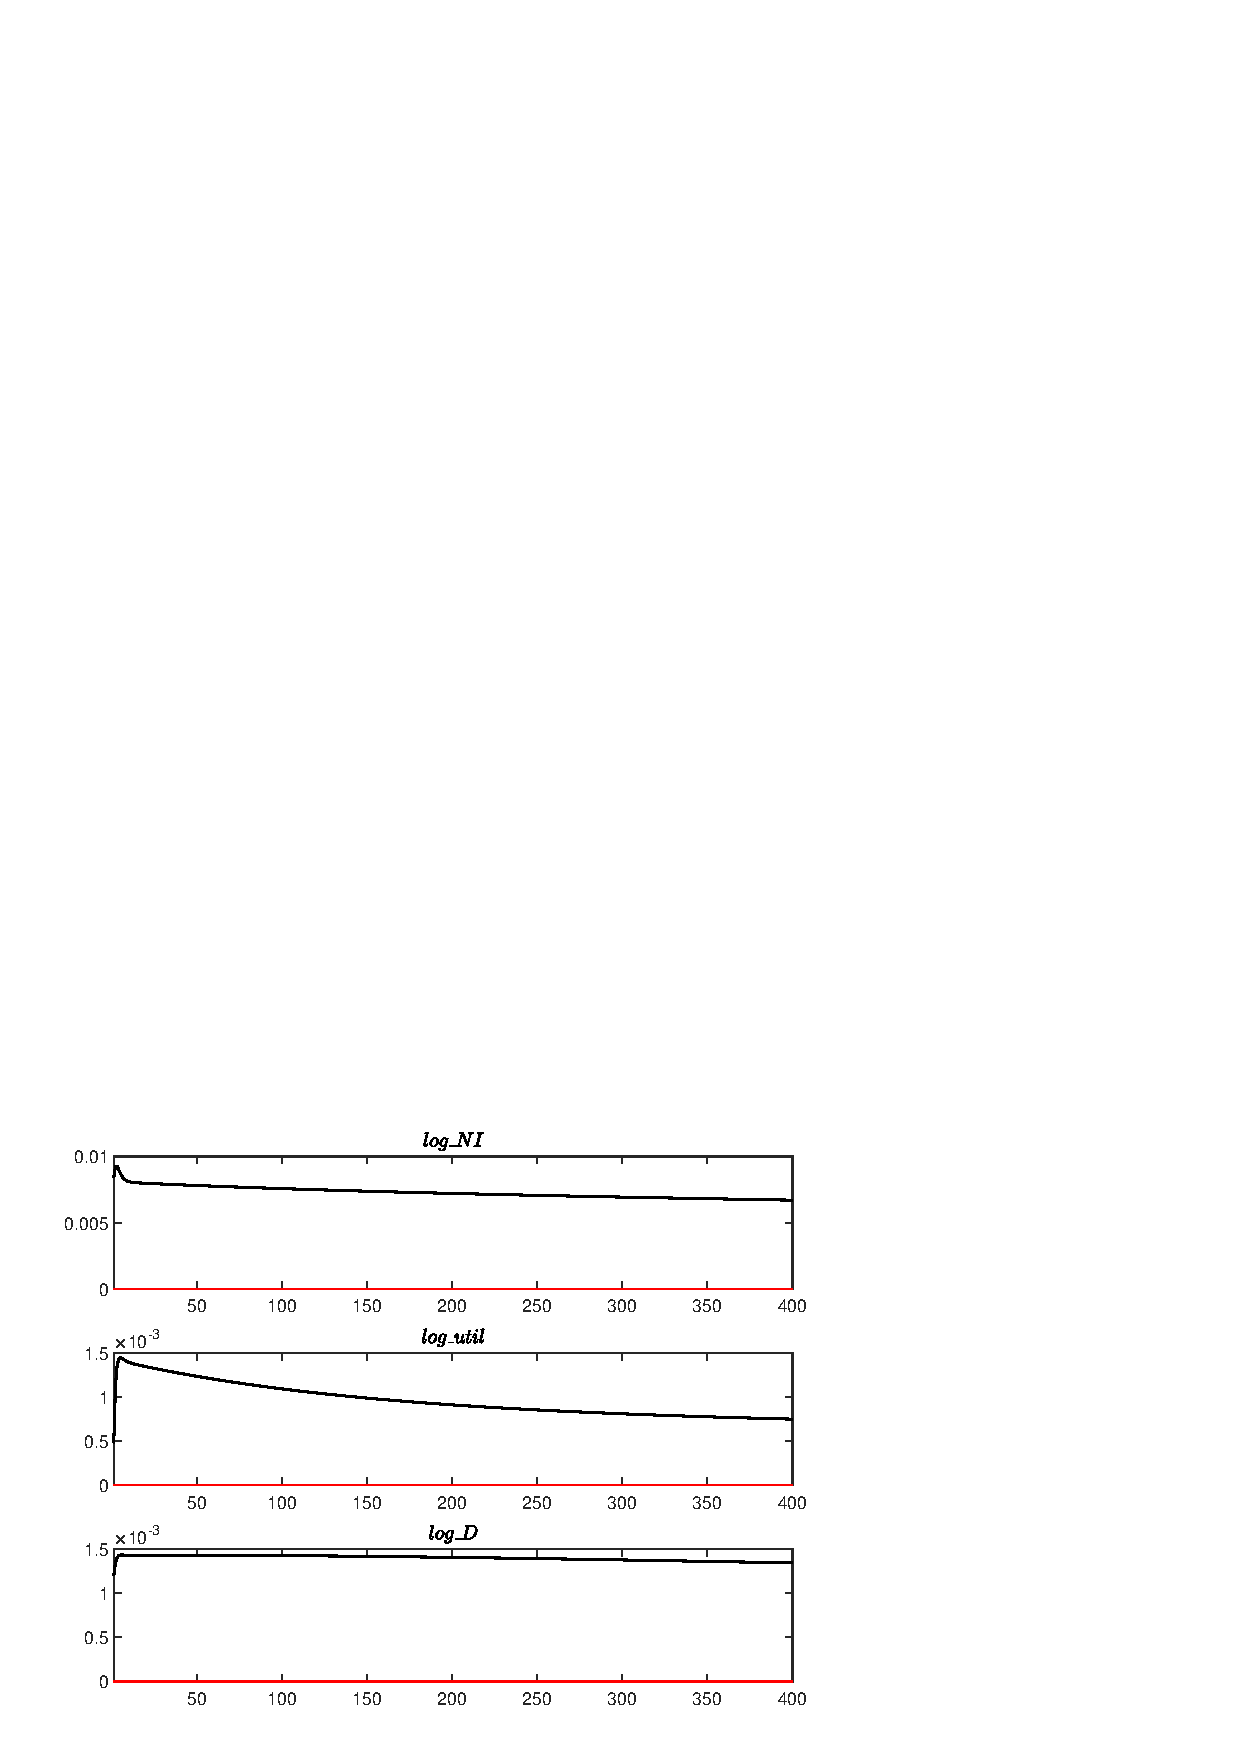
\includegraphics[width=0.80\textwidth]{BRS_growth/graphs/BRS_growth_IRF_e_C3}
\caption{Impulse response functions (orthogonalized shock to ${e_C}$).}\label{Fig:IRF:e_C:3}
\end{figure}
 
 
% End Of TeX file. 
